\documentclass[11pt]{article}
\usepackage[T1]{fontenc}
\usepackage[utf8]{inputenc}
\usepackage{lmodern}
\usepackage[margin=1in]{geometry}
\usepackage{amsmath,amssymb,amsthm,mathtools}
\usepackage{microtype}
\usepackage{enumitem}
\usepackage{tikz}
\usetikzlibrary{arrows.meta,calc}
\usepackage{url}
\usepackage[colorlinks=true,linkcolor=blue!45!black,citecolor=blue!45!black,urlcolor=blue!45!black]{hyperref}
\hypersetup{pdftitle={A continuum temperature singularity for a radial pair potential},pdfauthor={OpenAI}}
\newcommand{\R}{\mathbb R}
\newcommand{\N}{\mathbb N}
\newcommand{\eps}{\varepsilon}
\newcommand{\T}{T}
\newcommand{\dd}{\,\mathrm d}
\DeclareMathOperator{\conv}{conv}
\DeclareMathOperator{\supp}{supp}
\DeclareMathOperator{\dist}{dist}
\DeclareMathOperator{\diam}{diam}
\DeclareMathOperator{\Vol}{Vol}
\newtheorem{theorem}{Theorem}[section]
\newtheorem{proposition}[theorem]{Proposition}
\newtheorem{lemma}[theorem]{Lemma}
\newtheorem{corollary}[theorem]{Corollary}
\theoremstyle{definition}
\newtheorem{definition}[theorem]{Definition}
\theoremstyle{remark}
\newtheorem{remark}[theorem]{Remark}
\numberwithin{equation}{section}
\setlength{\emergencystretch}{1.5em}
\title{A continuum temperature singularity\protect\\for a radial pair potential}
\author{OpenAI}
\date{September 24, 2026}
\begin{document}
\maketitle
\begin{abstract}
We construct a stable radial pair potential in three dimensions whose canonical
free energy has a strict downward derivative jump at one common finite positive
inverse temperature throughout an open interval of positive densities. The
potential has a divergent repulsive core, a nontrivial attractive interval,
and an integrable tail satisfying $\phi(r)=o(r^{-3})$. Its free-cube canonical
free energy is finite at every positive inverse temperature and density.
\end{abstract}
\begingroup
\small
\tableofcontents
\endgroup
\clearpage
\section{The continuum existence problem}\label{sec:introduction}
A phase transition in a continuum particle system can be expressed as a loss of
regularity of its thermodynamic free energy. We consider an existence problem:
can a single species of particles in $\R^3$, interacting through a stable radial
pair potential, have a temperature singularity at one fixed density, and can the same
critical inverse temperature work throughout an open interval of densities?
We use the following precise class of potentials and normalization.

A potential $\Phi(x)=\phi(|x|)$ is \emph{admissible} if it is Borel measurable,
$\Phi(0)=+\infty$, and $\phi$ is finite and locally bounded on $(0,\infty)$,
with the following properties:
\begin{enumerate}[label=(\roman*),leftmargin=*]
\item $\phi(r)\to+\infty$ as $r\downarrow0$;
\item there are $0<r_1<r_2$ and $a>0$ such that
      $\phi(r)\le-a$ for every $r\in[r_1,r_2]$;
\item $\int_R^\infty r^2|\phi(r)|\dd r<\infty$ for some finite $R$;
\item there is $B<\infty$ such that, for every finite configuration,
\begin{equation}\label{eq:stability-target}
 U_N^\Phi(x_1,\ldots,x_N):=\sum_{1\le i<j\le N}\Phi(x_i-x_j)\ge-BN.
\end{equation}
\end{enumerate}
Let $\Lambda_L=[-L/2,L/2]^3$. With free boundary conditions, define
\begin{equation}\label{eq:canonical-definition}
 Z_{\Lambda,N}^{\Phi}(\beta)=\frac1{N!}
 \int_{\Lambda^N}e^{-\beta U_N^\Phi(x_1,\ldots,x_N)}
 \dd x_1\cdots\dd x_N,\qquad \beta>0,
\end{equation}
where $Z_{\Lambda,0}^{\Phi}=1$ and $e^{-\beta\infty}=0$. The position
measure is Lebesgue measure, independent of $\beta$; no temperature-dependent
normalization is included.
For a density $\rho>0$, the canonical free-energy density is
\begin{equation}\label{eq:free-energy-definition}
 f_\Phi(\beta,\rho)=-\frac1\beta
 \lim_{L\to\infty}L^{-3}\log
 Z_{\Lambda_L,\lfloor\rho L^3\rfloor}^{\Phi}(\beta),
\end{equation}
when the limit exists. The problem is to find an admissible $\Phi$ and a fixed
$\rho$ for which this limit is finite on an interval of positive inverse
temperatures and fails to be $C^1$ across an interior point.

Write $D_\beta^-$ and $D_\beta^+$ for the left and right derivatives
with respect to inverse temperature.

\begin{theorem}\label{thm:main}
There exist an admissible radial difference-only pair potential
$\Phi(x)=\phi(|x|)$ on $\R^3$, a nonempty open interval
$I\subset(0,\infty)$, and one $\beta_c\in(1/2,3/2)$ with the following
properties. The potential satisfies $\phi(r)=o(r^{-3})$ as $r\to\infty$.
The free-cube limit \eqref{eq:free-energy-definition} exists and is finite
for every $\beta>0$ and every density $\rho>0$. For every $\rho\in I$,
the finite one-sided derivatives at the same critical point satisfy
\[
 D_\beta^- f_\Phi(\beta_c,\rho)
 >D_\beta^+ f_\Phi(\beta_c,\rho).
\]
Thus one potential and one critical inverse temperature give a strict
canonical temperature singularity throughout $I$.
\end{theorem}

The construction uses a narrow low-energy shell inside a repulsive core,
together with a summable family of radial attractions at successively larger
ranges. Thus the theorem concerns an engineered potential in the explicit
integrable-tail class above. It does not assert a transition for the ordinary
$12$--$6$ Lennard--Jones potential, and it makes no identification of the
coexisting states as conventional liquid, vapor, or solid phases.

\subsection{Context and the role of the fixed density}
The continuum phase-transition existence question belongs to the program
highlighted by Simon's problems in mathematical physics~\cite{Simon1984}.
Here the tail hypothesis is exactly condition~(iii). The construction also
gives $\phi(r)=o(r^{-3})$, but does not establish a bound
$|\phi(r)|\le C r^{-3-\varepsilon}$ with any fixed $\varepsilon>0$.
Accordingly, the theorem does not claim to resolve formulations of the
historical problem that require such a power-law margin.

Earlier rigorous continuum transitions include Ruelle's result for the
two-species Widom--Rowlinson model~\cite{Ruelle1971}. Israel's convex
construction also applies to hard-core continuum particles: a
spherically symmetric pair perturbation and a chemical potential produce
two invariant equilibrium states of different densities
\cite[Section~6, Theorem~8(a)]{Israel1975}.
The hard core in that result excludes a positive interval of separations;
the potential constructed here is finite at every positive separation.
Lebowitz, Mazel, and Presutti later proved a transition for a model with
attractive pair and repulsive four-body interactions
\cite{LebowitzMazelPresutti1998,LebowitzMazelPresutti1999}.
The four-body term remains part of that model.

Recent constructions impose other structures on the interaction.
He, Jauslin, Lebowitz, and Peled prove distinct-density Gibbs coexistence
for suitable parameters and sufficiently large range in a model with a
box-modified Kac pair interaction
\cite[Equation~(1.13) and Theorem~1.3]{HeJauslinLebowitzPeled2025}.
It depends on a fixed partition into cubes, and the reference interaction
acts only within each cube. Dereudre and Renaud-Chan prove
low-temperature coexistence for saturated finite-range interactions
satisfying a Peierls condition~\cite[Theorem~1]{DereudreRenaudChan2026}.
Their radial-kernel example integrates over unions of particle
neighborhoods, giving a many-body energy rather than an ordinary pair sum
\cite[Section~2.3, Example~3, Equation~(2.18)]{DereudreRenaudChan2026}.
Our final interaction is a radial function of the particle difference,
with all cross-cube interactions retained. Moreover, density coexistence
alone does not imply a temperature corner at a fixed density. We obtain
two supporting slopes with the same density coordinate and different
energy coordinates, the information needed for the strict derivative
jump in~\eqref{eq:free-energy-definition}.

The long-range comparison is a version of the Lebowitz--Penrose
mean-field limit~\cite{LebowitzPenrose1966}; its extension to superstable
interactions is classical~\cite{GerardiEtAl1973}. Our estimates include
local occupation and tail-continuity bounds uniform in the previously
chosen attraction ranges. The Kac limit itself fixes each finite reference
before sending the new range to infinity. The local quadratic energy
estimates belong to Ruelle's superstability framework~\cite{Ruelle1970}.
Convex methods for constructing coexistence have antecedents in
Israel's tangent-functional argument~\cite[Theorem~1]{Israel1975}
and Ruelle's restoration of lattice-gas coexistence by small changes of
long-range pair couplings and chemical potential
\cite[Section~5]{Ruelle1977Coexistence}.
Here the scaled perturbation argument keeps three separated groups of
joint pressure slopes, and hence a common ball of slopes, through
infinitely many physical approximations.

A companion construction~\cite[Theorem~1.1]{OpenAIAlgebraic2026}
gives a bounded continuous radial potential with
$|\phi(r)|\le Cr^{-3-1/32}$ for $r\ge1$ and a common temperature
singularity throughout a density interval.
That result uses a different potential and a quantitative range estimate;
the present proof retains the divergent core and proves its own
integrable-tail conclusion.


\subsection{How the construction works}
For orientation, fix a scale $t>0$ and write the activity as $e^{th}$.
The normalized pressure is the thermodynamic limit of
\[
 \frac1{tL^3}\log\sum_{N\ge0}e^{thN}Z_{\Lambda_L,N}^\Phi(\beta).
\]
It is a convex function of $(\beta,h)$. A supporting vector $(s,d)$ at
$(\beta_0,h_0)$ gives an affine plane of slope $(s,d)$ lying below that
function and touching it there. The coordinate $d$ represents density.
The proof will preserve a two-dimensional ball of these vectors, so that
one density is compatible with more than one first-coordinate slope.

The proof follows four steps.
\begin{enumerate}[leftmargin=*]
\item \textbf{Build a stable reference gas.}
The core allows pairs at an extremely small separation shell at no energy
cost. At most four particles can have all their pair distances in that shell
in $\R^3$. This geometric fact supplies a quadratic local lower bound for the
energy. Section~\ref{sec:model} uses that bound to establish the canonical
thermodynamic limit and its dual grand-canonical pressure. The scaled
function $\beta f_\Phi(\beta,\rho)/t$ is concave in inverse temperature.
\item \textbf{Create three competing pressure branches.}
For a large scale parameter $t$, the grand-canonical activity is $e^{th}$.
The reference pressure has three limiting branches, corresponding to empty
space, well-separated particles, and tetrahedral clusters. Adding a spread-out radial attraction contributes a positive quadratic
density term to the variational formula for pressure. Sections~\ref{sec:kac}
and~\ref{sec:triple} establish this comparison and produce a pressure with
three noncollinear groups of supporting slopes.
\item \textbf{Preserve those slopes at finite ranges.}
Uniform approximation alone can smooth a corner. Section~\ref{sec:convex}
therefore works at the scale of each new attractive mass: the physical
approximation error is smaller than that scale, while the density quadratic
separates the three groups. At each stage this yields a nearby point with the
same ball of supporting slopes.
\item \textbf{Pass to one potential and a density interval.}
Section~\ref{sec:construction} chooses the attraction masses before the
corresponding approximation ranges. Their summability gives one admissible
potential, and summable shifts give one limiting pressure point. The common
ball of supporting slopes passes to that physical pressure. Every horizontal slice near the center of the ball fixes a positive
density and gives two different inverse-temperature slopes of the canonical
free energy at the same critical point.
\end{enumerate}

The elementary convex facts used in these steps are proved in
Appendix~\ref{app:convex-facts}. They include local uniform convergence,
partial conjugacy, and representation of a subdifferential by limits of
ordinary gradients.

\section{A stable class with four-particle clusters}
\label{sec:model}

We first construct a class of potentials for which thermodynamic limits
exist and the required density bounds are uniform in the ranges of the
attractive interactions.
The positive core permits small clusters of at most four particles without
an energy cost. Its quadratic penalty for larger local populations will
control every attractive term added later.

\subsection{The packing density and the core}

Let $M_L$ be the largest cardinality of a subset of
$\Lambda_L=[-L/2,L/2]^3$ whose distinct points have distance at least one.
The number is finite, and compactness gives a maximizing configuration.
There is a constant
\begin{equation}
 p=\lim_{L\to\infty}\frac{M_L}{L^3}\in(0,\infty),
 \qquad A=\frac{3}{2p}.
 \label{eq:packing-density}
\end{equation}
Here we need only the existence of $p$, not its numerical value. Disjoint
balls of radius $1/2$ around the packing points lie in the cube of side
$L+1$, giving an upper bound on $M_L/L^3$ for $L\ge1$. A unit lattice
gives a positive lower bound. For convergence, repeat a maximizing packing
in a cube of side $s$ with period $s+1$ in each coordinate. Points in
different copies are still separated by at least one, so
\[
 \liminf_{L\to\infty}\frac{M_L}{L^3}
 \ge \frac{M_s}{(s+1)^3}.
\]
Letting $s\to\infty$ along a sequence realizing the limsup proves
\eqref{eq:packing-density}.

Fix
\[
 \delta=10^{-3},\qquad b=\frac14.
\]
For a parameter $t>1$, put $E=t^2$ and $e_t=e^{-t}$. Define the radial
nonnegative core, with $r=|x|$, by
\begin{equation}
 \psi_t(x)=
 \begin{cases}
 +\infty,&r=0,\\
 E+(e_t/r)^{12},&0<r<e_t,\\
 0,&e_t\le r\le(1+\delta)e_t,\\
 E,&(1+\delta)e_t<r<1,\\
 0,&r\ge1.
 \end{cases}
 \label{eq:core}
\end{equation}
Thus particles can approach one another without paying the energy $E$
only when their separation lies in a narrow shell of radius $e_t$.
We allow $t$ to vary until the initial pressure configuration has been
constructed; thereafter one sufficiently large finite value will be fixed.

Choose a nonnegative radial function $w\in C^1(\R^3)$, supported in the
unit ball, strictly positive on the closed ball of radius $1/2$, and
normalized by $\int_{\R^3}w(x)\,\dd x=1$. For $R\ge1$ set
$w_R(x)=R^{-3}w(x/R)$. Our class consists of
\begin{equation}
 \varphi=\psi_t-S,
 \qquad S=t\sum_j\sigma_j w_{R_j},
 \qquad R_j\ge1,\quad \sigma_j\ge0,
 \quad \sum_j\sigma_j\le A+1.
 \label{eq:physical-class}
\end{equation}
The sum may be finite, empty, or countably infinite. Since
$\|w_R\|_\infty\le\|w\|_\infty$ and $\|w_R\|_1=1$, it converges
uniformly and in $L^1$ in the infinite case. In particular, $S$ is a
bounded continuous nonnegative function. Every potential in this class is
nonpositive at distances at least one. This sign will give a direct proof
of the canonical thermodynamic limit.

Partition $\R^3$ into half-open cubes $C_i$ of side $b$, indexed by
$i\in\mathbb Z^3$. For a finite configuration, let $n_i$ be the number
of its particles in $C_i$. In a finite cube we intersect these cells with
the cube; every resulting cell has volume at most $b^3$. Set
\begin{equation}
 J_{ij}=\sup_{x\in C_i,\,y\in C_j}S(x-y),
 \qquad \sum_jJ_{ij}\le M,
 \qquad M=c_b t(A+1),
 \label{eq:cell-row}
\end{equation}
where $c_b$ depends only on $b$ and $w$. To see the row bound, first use
one kernel $w_R$. Each nonzero cell supremum is at most
$\|w\|_\infty R^{-3}$, and there are at most $C_bR^3$ cells within
distance $R$ of a given cell because $R\ge1$. Sum this bound over the
coefficients $t\sigma_j$. Taking a supremum of a sum only decreases the
result relative to the sum of suprema. The same proof therefore applies
to infinitely many ranges and to cropped cells.

\begin{lemma}[The shell graph]
\label{lem:shell-graph}
No five points in $\R^3$ have all their mutual distances in
$[e_t,(1+\delta)e_t]$. Consequently, a graph whose vertices are points
of $\R^3$ and whose edges join pairs at these distances has at most
$3n^2/8$ edges on any set of $n$ vertices.
\end{lemma}

\begin{proof}
Suppose that five such points existed. Scale by $e_t^{-1}$ and form the
Gram matrix $G$ of the four vectors from one point to the other four.
Write $\varepsilon=2\delta+\delta^2$. The diagonal entries differ
from 1 by at most $\varepsilon$. By the polarization identity, each
off-diagonal entry differs from $1/2$ by at most $\varepsilon$.
The matrix $G_0$ with diagonal 1 and off-diagonal $1/2$ has smallest
eigenvalue $1/2$, whereas
\[
 \|G-G_0\|_{\mathrm{op}}\le4\varepsilon
 =0.008004<\frac12.
\]
Thus $G$ would have rank four, which is impossible for four vectors
in $\R^3$.

For completeness, we give the weighted proof of the required graph bound,
an instance of the Motzkin--Straus identity
\cite[Theorem~1]{MotzkinStraus1965}.
For a graph with no complete subgraph on five vertices, maximize
\[
 \sum_{\{i,j\}\text{ an edge}}a_i a_j
 \quad\text{over}\quad a_i\ge0,\qquad\sum_i a_i=1.
\]
Choose a maximizer with the smallest possible support. If two vertices
in its support are nonadjacent, transferring all their combined weight
to the one with the larger weighted neighbor sum cannot decrease the
objective. It decreases the support, a contradiction. The support is
therefore a clique with at most four vertices. At this maximizer the
objective is
\[
 \frac12\left(1-\sum_i a_i^2\right)\le\frac38.
\]
Applying this inequality to the weights $a_i=1/n$ gives the asserted
edge count. The case $n=0$ is immediate.
\end{proof}

\begin{proposition}[Uniform stability]
\label{prop:stability}
Put $A_0=E/8$ and $B_0=E/2$. Every potential in
\eqref{eq:physical-class} satisfies, for every finite configuration,
\begin{equation}
 \sum_{\ell<k}\psi_t(x_\ell-x_k)
 \ge A_0\sum_i n_i^2-B_0N,
 \qquad
 U_N^\varphi\ge (A_0-M/2)\sum_i n_i^2-B_0N.
 \label{eq:superstable}
\end{equation}
These inequalities remain valid if positive core interactions between
members of a partition into unions of whole cells are deleted, or if
any negative interactions are multiplied by factors in $[0,1]$.
\end{proposition}

\begin{proof}
The diameter of a cell is $\sqrt3/4<1$. Among the $n_i(n_i-1)/2$
pairs inside cell $i$, at most $3n_i^2/8$ lie in the shell by
Lemma~\ref{lem:shell-graph}. Every other pair has core energy at
least $E$. Thus the core energy inside this cell is at least
\[
 E\left(\frac{n_i(n_i-1)}2-\frac{3n_i^2}8\right)
 =A_0 n_i^2-B_0 n_i.
\]
All remaining core interactions are nonnegative. Also,
\[
 \sum_{\ell<k}S(x_\ell-x_k)
 \le\frac12\sum_{i,j}J_{ij}n_i n_j
 \le\frac M2\sum_i n_i^2,
\]
where the first bound includes harmless self-particle terms and the
second follows from symmetry, \eqref{eq:cell-row}, and
$2n_i n_j\le n_i^2+n_j^2$. This proves
\eqref{eq:superstable}. The permitted deletions preserve every core
interaction within a small cell. Reducing a negative term only
increases the energy, so the same argument proves the last assertion.
\end{proof}

From now on we require $t$ to be sufficiently large that
\begin{equation}
 2(1+\delta)e_t<1,
 \qquad A_0\ge8M,
 \qquad \kappa:=(A_0-M/2)b^3>10t(A+1).
 \label{eq:t-choice}
\end{equation}
These conditions hold for all sufficiently large $t$, since $A_0$ is
quadratic in $t$ and $M$ is linear in $t$. In particular every potential
in the class is stable with constant $B_0$.

Each such potential is finite and locally bounded away from the origin
and diverges to $+\infty$ there. Its tail is integrable, since
$\varphi=-S$ outside the unit ball. If one coefficient is positive
and its range is greater than 4, the potential is strictly negative
uniformly on $1\le |x|\le2$: the corresponding rescaled kernel has
a positive minimum there, while the core vanishes. Thus a potential
with this additional simple condition has all the admissibility
properties in the introduction. We next establish its thermodynamics,
uniformly for the larger class \eqref{eq:physical-class}.

\subsection{The canonical limit for every density}

Fix for the moment a value of $t$ satisfying \eqref{eq:t-choice} and
a potential $\varphi$ in \eqref{eq:physical-class}. Write
$Z_{L,n}(\beta)=Z_{\Lambda_L,n}^\varphi(\beta)$, including
$Z_{L,0}=1$, and set
\[
 a_L(\beta,n)=-\frac{\log Z_{L,n}(\beta)}{tL^3}.
\]
We use $0\log0=0$. The following proposition includes convergence
along every sequence of particle numbers with a prescribed limiting
density; that form will be needed in the long-range comparison.

\begin{proposition}[Canonical and grand-canonical limits]
\label{prop:thermodynamics}
For every $\beta>0$ and $d\ge0$ there is a finite limit
\begin{equation}
 H_\varphi(\beta,d)
 =-\lim_{\substack{L\to\infty\\n/L^3\to d}}
       \frac{\log Z_{L,n}(\beta)}{tL^3},
 \qquad H_\varphi(\beta,0)=0.
 \label{eq:canonical-limit}
\end{equation}
Extend $H_\varphi(\beta,d)$ by $+\infty$ for $d<0$. It is closed
and convex in $d$, and finite and concave in $\beta$ for every
$d\ge0$. Moreover,
\begin{equation}
 H_\varphi(\beta,d)
 \ge \frac{\beta\kappa}{t}d^2
       -\frac{\beta B_0}{t}d
       +\frac{d\log d-d}{t}
 \qquad(d\ge0).
 \label{eq:coercivity}
\end{equation}
Let $\Omega=(0,\infty)\times\R$, with coordinates $(\beta,h)$,
and define
\[
 \Xi_L^\varphi(\beta,h)
   =\sum_{n\ge0}e^{thn}Z_{L,n}(\beta).
\]
Then the finite convex pressure is
\begin{equation}
 Q_\varphi(\beta,h)
 =\lim_{L\to\infty}\frac{\log\Xi_L^\varphi(\beta,h)}{tL^3}
 =\sup_{d\ge0}\{hd-H_\varphi(\beta,d)\}.
 \label{eq:pressure-duality}
\end{equation}
The convergence is uniform on compact subsets of $\Omega$, and
\begin{equation}
 H_\varphi(\beta,d)
 =\sup_{h\in\R}\{hd-Q_\varphi(\beta,h)\}
 \qquad(d\in\R).
 \label{eq:partial-conjugacy}
\end{equation}
The bounds above use the same constants for the entire class
\eqref{eq:physical-class} with the chosen $t$.
\end{proposition}

\begin{proof}
We give the details of the canonical limit first. Two finite-volume
bounds control the density adjustments in its construction.

\emph{A trial bound on bounded density intervals.}
Fix $D_0<\infty$ and choose a grid spacing $q\in(0,1/2)$ with
$q^{-3}>D_0+1$. For large $L$, at least $D_0L^3$ grid centers lie
in $\Lambda_L$ at distance $q/8$ from its boundary. For
$n\le D_0L^3$, put one particle in each of $n$ distinct balls of
radius $q/8$ around such centers. Every pair has distance at least
$3q/4$, and each particle has at most $Cq^{-3}$ neighbors at distance
less than one. The core is bounded on $[3q/4,1]$, so the positive
energy of these configurations is at most $E_q n$ for a finite
constant $E_q$. We need not count the negative energy. The $n!$
assignments of the labeled particles to the balls have disjoint
integration regions and cancel the canonical factorial. If $v_q>0$
is the volume of a ball, this gives
\[
 Z_{L,n}(\beta)\ge v_q^n e^{-\beta E_q n}.
\]
Consequently
\begin{equation}
 a_L(\beta,n)\le C_{D_0,\beta}
 \qquad(0\le n\le D_0L^3, L\text{ sufficiently large}).
 \label{eq:trial-bound}
\end{equation}
The constant is uniform over the physical class, and can be chosen
uniformly for $\beta$ in a compact subset of $(0,\infty)$.

\emph{A lower bound.}
There are at most $(L/b+2)^3$ cropped cells in $\Lambda_L$.
Cauchy--Schwarz in \eqref{eq:superstable} and the inequality
$n!\ge(n/e)^n$ therefore give, with $d_L=n/L^3$,
\begin{equation}
 a_L(\beta,n)
 \ge \frac{\beta\kappa}{t(1+2b/L)^3}d_L^2
       -\frac{\beta B_0}{t}d_L
       +\frac{d_L\log d_L-d_L}{t}.
 \label{eq:finite-coercivity}
\end{equation}
Dropping the positive quadratic term also gives the same inequality
with only its last two terms. In particular, $Z_{L,n}$ is positive
and finite, and $a_L$ is bounded above and below when the density
stays in a fixed bounded interval and $L$ is large.

\emph{Convergence at a positive density.}
Fix $\beta>0$ and $d>0$. The increasing infima
\[
 I_j=\inf\left\{a_L(\beta,n):
       L\ge j,\ \left|n/L^3-d\right|\le1/j\right\}
\]
converge to a finite number $I$. Select $\ell_j\ge j$ and $n_j$
in this set such that $a_{\ell_j}(\beta,n_j)\le I_j+1/j$.
Then $n_j/\ell_j^3\to d$ and
$a_{\ell_j}(\beta,n_j)\to I$. Every sequence with
$L\to\infty$ and $n/L^3\to d$ has liminf at least $I_j$ for
each $j$, and hence at least $I$.

To prove the reverse inequality, tile part of a large cube by
\[
 k=\left\lfloor\frac{L}{\ell_j+2}\right\rfloor^3
\]
cubes of side $\ell_j$, leaving gaps of width two. Every interaction
between distinct cubes is nonpositive. For any prescribed counts
$m_1,\ldots,m_k$, restricting the integral to these cubes gives
\begin{equation}
 Z_{L,\sum_i m_i}(\beta)
 \ge\prod_{i=1}^k Z_{\ell_j,m_i}(\beta).
 \label{eq:separated-boxes}
\end{equation}
Indeed there are $(\sum_i m_i)!/\prod_i m_i!$ assignments of labels
to the cubes, and these give exactly the factorials on the right.

Start with $n_j$ particles in every small cube. Define a higher count
$n_{\mathrm{hi}}=\lfloor(4d+4)\ell_j^3\rfloor$ and the diluted
densities
\[
 d_b=\frac{n_j}{(\ell_j+2)^3},\qquad
 d_{\mathrm{hi}}=\frac{n_{\mathrm{hi}}}{(\ell_j+2)^3}.
\]
For large $j$, $n_j>0$, $n_{\mathrm{hi}}>n_j$, and
$d_b\to d$, $d_{\mathrm{hi}}\to4d+4$. If a target count $n$
exceeds $kn_j$, change some cubes to $n_{\mathrm{hi}}$; if it is
smaller, empty some cubes. One additional intermediate count realizes
$n$ exactly. For fixed sufficiently large $j$, this is possible for
all large $L$ with $n/L^3\to d$. The limiting upper fraction of
changed cubes is at most
\[
 c_j=\max\left\{
 \frac{(d-d_b)_+}{d_{\mathrm{hi}}-d_b},
 \frac{(d_b-d)_+}{d_b}\right\},
 \qquad c_j\longrightarrow0.
\]
All new counts are bounded by $(4d+4)\ell_j^3$, so their values of
$a_{\ell_j}$ have a common upper bound by \eqref{eq:trial-bound}.
The baseline values are bounded in absolute value. Applying
\eqref{eq:separated-boxes}, taking the large-volume limit with $j$
fixed, and then letting $j\to\infty$ therefore gives
\[
 \limsup_{\substack{L\to\infty\\n/L^3\to d}}a_L(\beta,n)
 \le\lim_{j\to\infty}
 \left(\frac{\ell_j}{\ell_j+2}\right)^3
 \bigl(a_{\ell_j}(\beta,n_j)+C c_j\bigr)=I.
\]
The single intermediate cube contributes zero in the first limit.
This proves the all-sequence convergence for $d>0$.

\emph{Zero density and convexity.}
When $n/L^3\to0$, the linear lower bound derived above has limit
zero. For an upper bound, fix a sufficiently large side $\ell$ and
use separated cubes as in \eqref{eq:separated-boxes}, with empty
baseline. Fill some cubes with $\lfloor\ell^3\rfloor$ particles
and at most one with an intermediate count. Their number is
$o(L^3)$, so \eqref{eq:trial-bound} gives a limiting upper bound
zero. Thus $H_\varphi(\beta,0)=0$.

For convexity, take $0\le d_1<d_2$ and a density strictly between
them. For a large fixed $\ell$, use counts
$\lfloor d_1\ell^3\rfloor$ and $\lfloor d_2\ell^3\rfloor$
in the separated cubes. The desired density lies strictly between
their diluted densities for all sufficiently large $\ell$.
Choose their proportions to attain the target count, with at most
one intermediate cube. Inequality~\eqref{eq:separated-boxes},
followed first by $L\to\infty$ and then by $\ell\to\infty$,
gives the convexity inequality for $H_\varphi(\beta,\cdot)$.
The endpoint cases of that inequality are immediate.

The function is finite and convex on $[0,\infty)$, hence continuous
on $(0,\infty)$. The linear lower bound gives lower
semicontinuity at zero; since its value there is zero, extension by
$+\infty$ to negative densities is a closed convex function.
For each fixed density, H\"older's inequality makes
$-\log Z_{L,n}(\beta)$ concave in $\beta$. Passage to the limit
gives finite concavity of $H_\varphi(\cdot,d)$ on $(0,\infty)$.
Finally \eqref{eq:finite-coercivity} gives
\eqref{eq:coercivity}.

We have established the canonical limit with enough control over
particle number to pass to the grand-canonical ensemble. In
particular, the density variable in the next maximization will not
require a separate approximation of the canonical free energy.

\emph{Pressure and conjugacy.}
On a compact subset of $\Omega$, \eqref{eq:finite-coercivity}
implies that, for sufficiently large $D$ and all large $L$,
\[
 e^{thn}Z_{L,n}(\beta)\le e^{-c n^2/L^3}
 \qquad(n>DL^3)
\]
with $c>0$ independent of the potential in the class. The sum of
these terms is exponentially small in $L^3$, whereas the term
$n=0$ is one. Among the remaining at most $\lfloor DL^3\rfloor+1$
terms, choose one of maximal size. Every subsequence has a further
subsequence on which its density converges to some $d\in[0,D]$.
The all-sequence canonical limit identifies the limiting exponent
as $hd-H_\varphi(\beta,d)$. Conversely, the term
$n=\lfloor dL^3\rfloor$ supplies this exponent as a lower bound
for every $d\ge0$. This proves \eqref{eq:pressure-duality}.

The finite-volume logarithms are finite and jointly convex in
$(\beta,h)$, by H\"older's inequality applied to their defining
integrals and sums. The limit is finite by the density bound, and
it is nonnegative because the empty configuration is allowed.
Lemma~\ref{lem:elementary-convex-convergence}, the finite-dimensional
convex convergence principle of \cite[Corollary~7.18]{RockafellarWets1998},
upgrades pointwise convergence
to uniform convergence on compact subsets of the open convex set
$\Omega$.
Finally, the closed convexity in density proved above permits the
one-dimensional Fenchel biconjugacy identity, proved in
Lemma~\ref{lem:elementary-conjugacy} and treated in
\cite[Theorem~11.1]{RockafellarWets1998}, yielding
\eqref{eq:partial-conjugacy}.
\end{proof}

\subsection{The quadratic density transform}

We will compare a physical pressure with the pressure obtained by
adding an attraction whose range tends to infinity. The appropriate
variational expression is a quadratic modification in the density
variable. For any physical pressure $Q=Q_\varphi$, write
\[
 H_Q(\beta,d)=\sup_{h\in\R}\{hd-Q(\beta,h)\}.
\]
By \eqref{eq:partial-conjugacy}, this is precisely the canonical
function $H_\varphi$, including its value $+\infty$ for $d<0$.
For $0\le\sigma\le A+1$, define
\begin{equation}
 (T_\sigma Q)(\beta,h)
 =\sup_{d\ge0}
   \left\{hd-H_Q(\beta,d)+\frac{\beta\sigma}{2}d^2\right\}.
 \label{eq:transform}
\end{equation}
This definition does not assert that $T_\sigma Q$ is itself the
pressure of a finite-range pair potential. The next section proves
the approximation by physical pressures that we shall use.

\begin{proposition}[Bounds for the density transform]
\label{prop:transform}
Let $t$ satisfy \eqref{eq:t-choice}. For every physical pressure
$Q_\varphi$ in \eqref{eq:physical-class} and every
$\sigma\in[0,A+1]$, the function $T_\sigma Q_\varphi$ is finite
and convex on $\Omega$, nonnegative, and nondecreasing in $h$.
The supremum in \eqref{eq:transform} is attained. For every compact
$W\subset\Omega$, there is $D_W<\infty$, depending only on
$W,t,b,w,A$, such that every maximizing density belongs to
$[0,D_W]$, uniformly over all potentials in the class and all these
values of $\sigma$. The transformed pressures are also uniformly
bounded on $W$.
\end{proposition}

\begin{proof}
The value at $d=0$ is zero. By \eqref{eq:coercivity}, the objective
in \eqref{eq:transform} is bounded above by
\begin{equation}
 hd-\beta\left(\frac\kappa t-\frac\sigma2\right)d^2
       +\frac{\beta B_0}{t}d
       -\frac{d\log d-d}{t}.
 \label{eq:transform-coercivity}
\end{equation}
Condition~\eqref{eq:t-choice} gives a uniform positive lower bound
on $\kappa/t-\sigma/2$. On a compact set of $(\beta,h)$ with
$\beta$ bounded away from zero, the right side is therefore
negative for every sufficiently large $d$, uniformly in the
potential and in $\sigma$. This proves the common density bound
and the finite upper bound for the supremum. The objective is upper
semicontinuous in $d$, since $H_Q(\beta,\cdot)$ is lower
semicontinuous. It attains its maximum on the resulting compact
interval.

For each fixed $d\ge0$, the function in braces in
\eqref{eq:transform} is convex in $(\beta,h)$: the canonical
function is concave in $\beta$, and the other terms are affine.
Their supremum is convex. Its monotonicity in $h$ follows from
$d\ge0$, and its nonnegativity from the zero-density choice.
\end{proof}

The normalizations are now fixed. In particular, for every positive
density the free energy in the statement of the problem is
\begin{equation}
 f_\varphi(\beta,d)=\frac{t}{\beta}H_\varphi(\beta,d).
 \label{eq:free-energy-normalization}
\end{equation}
For a real-valued function $F$ on a compact set $K$, write
$\|F\|_K=\sup_{x\in K}|F(x)|$.
All limits and finiteness statements in this section hold for every
$\beta>0$, including for infinite sums in
\eqref{eq:physical-class}. The remaining task is to choose the
attractive ranges and coefficients so that one of these canonical
functions has two different temperature slopes at one fixed
positive density.

\section{Uniform estimates and the Kac approximation}\label{sec:kac}

The next step relates a physical long-range attraction to the transform
\(\T_\sigma\) in \eqref{eq:transform}.  Throughout this section, \(t\) satisfies
\eqref{eq:t-choice} and is fixed.  All uniform estimates concern the physical
class \eqref{eq:physical-class} at this fixed \(t\); they need not remain
uniform as \(t\) tends to infinity.  The approximation is a form of the
Lebowitz--Penrose limit, whose extension to superstable reference interactions
is classical \cite{LebowitzPenrose1966,GerardiEtAl1973}.  We give the proof
because we will need constants independent of the attraction ranges, including
in auxiliary systems with some positive interactions removed.

\subsection{Local moments and continuity in the attractive tail}

Recall the cells \(C_i\) of side \(b\), their occupation numbers \(n_i\), and
the attractive interaction bounds \(J_{ij}\) from \eqref{eq:cell-row}.
In a finite cube, consider the grand canonical measure with activity \(e^{th}\).
We also allow two modifications: positive core interactions may be deleted
between boxes that are unions of whole cells, and negative pair interactions
may be multiplied by measurable symmetric factors in \([0,1]\).
Every original cell retains its internal core interaction.  Consequently,
the lower bound \eqref{eq:superstable} continues to hold.

\begin{proposition}[Uniform local moments]\label{prop:moments}
Fix a compact set \(\mathcal K\subset\Omega\).
For all potentials in \eqref{eq:physical-class}, all finite cubes, and all
the modified systems just described, there is a constant \(C_{\mathcal K}\)
such that
\[
 \mathbb E_{\beta,h}[n_i n_j]\le C_{\mathcal K}
 \qquad ((\beta,h)\in\mathcal K)
\]
for every pair of cells meeting the cube.  The constant is independent of
the number and ranges of the attractive summands.
\end{proposition}

\begin{proof}
Condition on the configuration \(Y\) outside \(C_i\), and put
\[
 A_i(Y)=\sum_{j\ne i}J_{ij}n_j,\qquad c=\frac{\beta A_0}{4}.
\]
The interactions involving the \(n\) particles inside \(C_i\) are bounded
below by
\[
 (A_0-J_{ii}/2)n^2-B_0n-nA_i.
\]
The empty cell contributes one to the conditional partition function.
Its volume is at most \(b^3\), also when cropped by the cube boundary.
It follows that
\begin{align*}
 \mathbb E[e^{c n_i^2}\mid Y]
 &\le
 \sum_{n\ge0}\frac{b^{3n}}{n!}
 \exp\!\left(cn^2+thn-\beta(A_0-J_{ii}/2)n^2
                  +\beta B_0n+\beta nA_i\right)\\
 &\le C_1\exp(\beta A_i^2/A_0).
\end{align*}
Indeed,
\(\beta nA_i\le\beta A_0n^2/4+\beta A_i^2/A_0\);
after this estimate the remaining negative quadratic coefficient is at least
\[
 \beta(A_0/2-M/2)\ge 7\beta A_0/16.
\]
The resulting one-variable series is bounded uniformly on \(\mathcal K\).
The conditional bound still depends on \(Y\).  We remove that dependence
by a finite-volume bootstrap.

Let \(F_i=\mathbb E[e^{c n_i^2}]\).  These numbers are finite before the
bootstrap: multiplying the grand canonical integrand by \(e^{cn_i^2}\)
leaves a strictly negative quadratic in all cell counts, by
\eqref{eq:superstable}.  Cauchy--Schwarz with weights \(J_{ij}\) gives
\[
 A_i^2\le M\sum_{j\ne i}J_{ij}n_j^2.
\]
If \(M>0\), set \(\theta_{ij}=J_{ij}/M\) and
\(\alpha=4(M/A_0)^2<1\).  Then $c\alpha=\beta M^2/A_0$. The row weights sum to at most one;
place any missing weight on a value zero. Convexity of the exponential and then
concavity of \(x^\alpha\) give
\[
 F_i\le C_1\left(1+\sup_j F_j^\alpha\right).
\]
There are finitely many cells, so their maximum is bounded by a constant
depending only on \(C_1,\alpha\).  When \(M=0\), the conditional estimate
already gives \(F_i\le C_1\).  Since \(\beta\) is bounded away from zero on
\(\mathcal K\), this proves uniform second moments.  A final
Cauchy--Schwarz inequality proves the assertion.
\end{proof}

This is a direct version of the local-occupancy estimates associated with
superstability \cite{Ruelle1970}.  Its extra uniformity will control both
the infinite tail and the boundary errors in the Kac comparison.

\begin{proposition}[Attractive perturbations]\label{prop:tail}
Fix a compact set \(\mathcal K\subset\Omega\).
For two of the preceding finite-volume systems differing by a negative
interaction, let \(J^{\mathrm{diff}}_{ij}\) be cellwise suprema of its
absolute value.  If the linear interpolation stays within the same
attractive mass bound, then
\begin{equation}\label{eq:pressure-interpolation}
 |\log\Xi(1)-\log\Xi(0)|
 \le \frac{\beta C_{\mathcal K}}2\sum_{i,j}J^{\mathrm{diff}}_{ij}
 \qquad ((\beta,h)\in\mathcal K).
\end{equation}
In particular, for
\[
 \varphi=\psi_t-t\sum_{j\ge1}\sigma_jw_{R_j},
 \qquad
 \varphi_n=\psi_t-t\sum_{j\le n}\sigma_jw_{R_j},
\]
there is a range-independent constant \(C'_{\mathcal K}\) such that
\begin{equation}\label{eq:tail-continuity}
 \|Q_\varphi-Q_{\varphi_n}\|_{\mathcal K}
 \le C'_{\mathcal K}\sum_{j>n}\sigma_j .
\end{equation}
\end{proposition}

\begin{proof}
Differentiate the logarithm of the grand partition function along the
interpolation.  The absolute derivative is at most
\[
 \frac{\beta}{2}\sum_{i,j}J^{\mathrm{diff}}_{ij}\,
                 \mathbb E[n_i n_j].
\]
Including particle self pairs only enlarges this bound.  Differentiation
under the integrals and sums is valid by the common negative quadratic
in the finitely many cell counts.  Proposition~\ref{prop:moments} and
integration over the interpolation parameter prove
\eqref{eq:pressure-interpolation}.

For the tail difference, each row sum is at most
\(c_b t\sum_{j>n}\sigma_j\), and the number of cells is at most
\((L/b+2)^3\).  Divide \eqref{eq:pressure-interpolation} by \(tL^3\),
use the pressure limit in Proposition~\ref{prop:thermodynamics}, and let
\(L\to\infty\).  The bounds are uniform on \(\mathcal K\), proving
\eqref{eq:tail-continuity}.
\end{proof}

\subsection{One long-range attraction}

\begin{proposition}[Physical Kac approximation]\label{prop:kac}
Let
\[
 \varphi=\psi_t-t\sum_{j=1}^k\sigma_jw_{R_j}
\]
have finitely many attractive summands, with the empty sum allowed.
Fix \(\sigma\ge0\) such that \(\sum_{j=1}^k\sigma_j+\sigma\le A+1\).
Then
\begin{equation}\label{eq:kac-limit}
 Q_{\varphi-t\sigma w_R}\longrightarrow\T_\sigma Q_\varphi
 \quad\text{as }R\to\infty
\end{equation}
uniformly on compact subsets of \(\Omega\).
\end{proposition}

\begin{proof}
Fix the reference potential, and let \(R_0\) bound its interaction range.
All constants depending on \(R_0\) are fixed during this proof.  Partition
a cube of side \(L=mu\) into \(m^3\) boxes of side
\[
 u=b\left\lfloor R^{1/2}/b\right\rfloor.
\]
Translate the \(b\)-cell lattice, if necessary, to align it with the
outside cube; all preceding estimates are invariant under this
translation.  The \(u\)-boxes are then unions of whole \(b\)-cells.
For each \(R\), we
first let \(m\to\infty\); only afterward do we let \(R\to\infty\).
In particular \(u\to\infty\), \(u/R\to0\), and eventually \(u\gg R_0\).

Write \(B_z\) for the box centered at \(z\), and define
\[
 K^+_{zz'}=\sup_{x\in B_z,\ y\in B_{z'}}w_R(x-y),
 \qquad
 K^-_{zz'}=\bigl(w_R(z-z')-Cu/R^4\bigr)_+.
\]
Choose the fixed constant \(C\) large enough that \(K^-_{zz'}\) is at most
the corresponding infimum.  The \(C^1\) bound on \(w\) and its compact
support imply, for some \(\eta_R=O(u/R)\to0\),
\begin{equation}\label{eq:kac-rows}
 u^3\sum_{z'}K^+_{zz'}\le1+\eta_R.
\end{equation}
If \(z\) is farther than \(R+3u\) from the outside cube boundary, then
\begin{equation}\label{eq:kac-lower-row}
 \sum_{z'}K^-_{zz'}\ge(1-\eta_R)u^{-3}.
\end{equation}
Here the sums are over the finite center grid in the cube.  To check these
estimates, compare \(u^3\sum_{z'}w_R(z-z')\) with \(\int w_R=1\).
The oscillation in each grid cube is \(O(uR^{-4})\), and only
\(O((R/u)^3)\) cubes meet the support enlarged by \(3u\).  The total
error after multiplication by \(u^3\) is \(O(u/R)\).
The same argument controls the suprema and the truncated lower kernel.
Also \(K^\pm_{zz'}\le C R^{-3}\).

\paragraph{Upper bound.}
Delete all positive core interactions between the \(u\)-boxes.  This
increases the partition function.  Remove next the reference attractive
interactions between these boxes, keeping the new Kac attraction in
place.  By Proposition~\ref{prop:tail}, this second change costs at most
\(C_{\mathcal K,R_0}L^3/u\) in the logarithm.  Indeed only original cells
within \(R_0+2b\) of a box boundary have a nonzero difference row, and
there are \(O_{R_0}(L^3/u)\) such cells.  Proposition~\ref{prop:moments}
applies throughout this interpolation.

Write \(n_z\) for the count in the box centered at \(z\).
The long-range pair sum is at most
\[
 \frac12\sum_{z,z'}K^+_{zz'}n_zn_{z'}
 \le \frac{1+\eta_R}{2u^3}\sum_z n_z^2,
\]
where the last step uses symmetry and
\(n_zn_{z'}\le(n_z^2+n_{z'}^2)/2\).
The first bound includes self pairs, which is harmless for this upper
estimate of an attractive Boltzmann factor.  The remaining reference
interactions are confined to individual boxes.  Summing the assignments
of particle labels cancels the global canonical factorial and gives
\begin{equation}\label{eq:kac-upper}
 \Xi_{mu}^{\varphi-t\sigma w_R}
 \le
 \exp(C_{\mathcal K,R_0}L^3/u)
 \left[
 \sum_{n\ge0}e^{thn}Z_{u,n}^{\varphi}(\beta)
 \exp\!\left(\frac{\beta t\sigma(1+\eta_R)}{2u^3}n^2\right)
 \right]^{m^3}.
\end{equation}

The finite-volume bound \eqref{eq:finite-coercivity} and
\(\kappa>10t(A+1)\) leave the effective energy coefficient
\[
 \frac{\kappa}{(1+2b/u)^3}-\frac{t\sigma(1+\eta_R)}2>0
\]
uniformly away from zero for all sufficiently large $R$. Consequently
counts \(n/u^3>D\), for sufficiently large \(D\), are suppressed by a
uniform negative quadratic.  The sum of
these high-count terms is exponentially small compared with the empty
term.  Among the remaining \(O(u^3)\) terms, every maximizing subsequence
has a further subsequence with \(n/u^3\to d\in[0,D]\).
The all-sequence limit \eqref{eq:canonical-limit} then gives
\[
 \lim_{R\to\infty}\frac1{tu^3}
 \log\!\left[
 \sum_{n\ge0}e^{thn}Z_{u,n}^{\varphi}(\beta)
 \exp\!\left(\frac{\beta t\sigma(1+\eta_R)}{2u^3}n^2\right)
 \right]
 =\sup_{d\ge0}\left\{hd-H_\varphi(\beta,d)
                         +\frac{\beta\sigma d^2}{2}\right\}.
\]
The logarithm of the number of low-count terms divided by \(u^3\)
vanishes.  This proves the equality by the preceding upper subsequence
argument and by taking \(n=\lfloor du^3\rfloor\) for the lower bound.
Taking first \(m\to\infty\) in \eqref{eq:kac-upper} and then \(R\to\infty\)
proves the desired upper estimate.

\paragraph{Lower bound.}
Place a cube of side \(s=u-2\) at each of the same centers, and require
exactly \(n=\lfloor ds^3\rfloor\) particles in every smaller cube,
where \(d\ge0\) is fixed.  The gaps have width two.  Thus all reference
interactions between distinct smaller cubes are nonpositive and can be
discarded in a lower bound on the partition function.
Let \(m_{\mathrm{int}}\) be the number of centers satisfying the
interior condition in \eqref{eq:kac-lower-row}.  The Kac pair sum obeys
\[
 \sum_{\ell<j}w_R(x_\ell-x_j)
 \ge \frac12m_{\mathrm{int}}n^2u^{-3}(1-\eta_R)
                      -\frac12m^3nCR^{-3}.
\]
The last term removes the particle self pairs included in the diagonal
box contribution.  The count constraint and the canonical factorials
therefore give
\begin{align*}
 \Xi_{mu}^{\varphi-t\sigma w_R}
 \ge{}&
 \left(e^{thn}Z_{s,n}^{\varphi}(\beta)\right)^{m^3}\\
 &{}\times
 \exp\!\left\{\frac{\beta t\sigma}{2}
 \left[m_{\mathrm{int}}n^2u^{-3}(1-\eta_R)-m^3nCR^{-3}\right]\right\}.
\end{align*}
For fixed \(R\), \(m_{\mathrm{int}}/m^3\to1\) as \(m\to\infty\).
Next \(R\to\infty\) gives \(s/u\to1\), \(n/s^3\to d\), and a vanishing
self-pair error.  By \eqref{eq:canonical-limit}, the resulting pressure
lower bound is
\[
 hd-H_\varphi(\beta,d)+\frac{\beta\sigma d^2}{2}.
\]
Take the supremum over \(d\ge0\).

We have proved pointwise convergence in \eqref{eq:kac-limit}.
The functions on both sides are finite and convex on the open convex
set \(\Omega\), by Propositions~\ref{prop:thermodynamics}
and~\ref{prop:transform}.  Pointwise convergence of finite convex
functions to a finite convex function is uniform on compact subsets,
which completes the proof.
\end{proof}

The proposition uses boxes only in its upper and lower estimates.
Both sides of \eqref{eq:kac-limit} are built from the full radial
reference interaction.  At every later stage we will fix the finite
reference first and then choose a sufficiently large new range; no
uniform rate over changing reference ranges is required.

\section{An initial triple of supporting slopes}\label{sec:triple}

We now choose \(t\) so that the ideal transform \(\T_AQ_{\psi_t}\)
has three separated groups of supporting slopes. The core permits
zero-energy clusters of sizes \(m=1,2,3,4\). After one root is positioned,
each of the other \(m-1\) particles has a relative position in a region
of volume proportional to \(e^{-3t}\). With activity \(e^{th}\), the
leading exponent per cluster, divided by \(t\), is therefore
\[
 mh-3(m-1).
\]
This expression is affine in \(m\), so its maximum over the four allowed
sizes occurs at \(m=1\) or \(m=4\). Using the limiting packing density
\(p\), together with the empty configuration, gives the three branches
in the next proposition. The proof below controls configurations that
pay a positive core energy as well.

\subsection{The free-cluster limit}

Write \(q_t=Q_{\psi_t}\).  In this section we temporarily let
\(t\to\infty\); one value will be fixed at its end.
The packing density \(p\) and \(A=3/(2p)\) retain their definitions
from Section~\ref{sec:model}.

\begin{proposition}[Reference pressure]\label{prop:free-pressure}
Uniformly on compact subsets of \(\Omega\),
\begin{equation}\label{eq:free-pressure-limit}
 q_t(\beta,h)\longrightarrow
 q_*(h):=\max(0,ph,4ph-9p).
\end{equation}
\end{proposition}

\begin{proof}
Call a configuration free if every pair distance below one lies in
\([e^{-t},(1+\delta)e^{-t}]\).  Join points at distance below one.
A two-edge path has endpoint distance at most
\(2(1+\delta)e^{-t}<1\); freeness makes the endpoints adjacent.
Thus connected components are complete graphs.
The geometric estimate in Lemma~\ref{lem:shell-graph} bounds
their sizes by four.  Representatives from different components
are separated by at least one, so their number is at most \(M_L\).

Let \(V=L^3\), and let \(\Xi_{\mathrm{free}}\) denote the grand
configurational integral restricted to free configurations.  Root
each component and integrate its root over volume \(V\).
Every other point in the component lies in a ball of volume at most
\(c_0e^{-3t}\) about the root.  The labeled block enumeration,
followed by division by the canonical factorial, gives the upper bound
\begin{equation}\label{eq:free-enumeration}
 \Xi_{\mathrm{free}}\le
 \sum_{k=0}^{M_L}\frac{(V\Theta_t)^k}{k!},
 \qquad
 \Theta_t=\sum_{m=1}^4
 \frac{e^{thm}(c_0e^{-3t})^{m-1}}{(m-1)!}.
\end{equation}
For completeness, ordered component sizes give a factor
\(1/(k!\prod m_i!)\); allowing any of the \(m_i\) labels to be a
root replaces \(m_i!\) by \((m_i-1)!\) and only increases the count.
Ignoring separation between the roots also enlarges the integral.

A bad edge is a pair at distance below one but outside the allowed
shell.  If there are \(B\) bad edges, their endpoint set \(S\) has
size at most \(2B\), its complement is free, and the core energy
is at least \(t^2B\).  Hence, pointwise on labeled configurations,
\[
 e^{-\beta U^{\psi_t}}
 \le \sum_{S\subset\{1,\ldots,N\}}
        e^{-\beta t^2|S|/2}\,
        {\bf1}_{\{\text{the complement of }S\text{ is free}\}}.
\]
The term corresponding to the actual bad-edge endpoint set proves
this inequality; zero Boltzmann factors cause no difficulty.
Summing over particle numbers and integrating the removed particles
gives
\begin{equation}\label{eq:bad-particle-factor}
 \Xi_L^{\psi_t}
 \le \exp\!\left(Ve^{th-\beta t^2/2}\right)\Xi_{\mathrm{free}}.
\end{equation}

Now
\[
 \frac1t\log\Theta_t
 \longrightarrow
 \max_{1\le m\le4}\{mh-3(m-1)\}
 =\max(h,4h-9).
\]
The convergence is uniform for bounded \(h\).  For \(u=k/V\),
the factorial estimate \(k!\ge(k/e)^k\) bounds the remaining
normalized logarithm in \eqref{eq:free-enumeration} by
\(u(1-\log u)/t\), with value zero at \(u=0\).
It is uniformly \(o(1)\) for bounded \(u\) as \(t\to\infty\).
There are only \(M_L+1=O(V)\) terms.
Take \(L\to\infty\) first and use \(M_L/V\to p\).
The extra pressure in \eqref{eq:bad-particle-factor} is
\(e^{th-\beta t^2/2}/t\), which tends to zero uniformly on compact
subsets of \(\Omega\).  This proves the upper limit in
\eqref{eq:free-pressure-limit}.

For the lower limit, fix \(\ell>0\) and \(\eta>0\).  Dilate an optimal
\(M_\ell\)-packing by \(1+\eta\), and repeat it with cubic period
\[
 P=(1+\eta)(\ell+2).
\]
In a cube of side \(mP\), the \(k=m^3M_\ell\) resulting centers have
mutual distances at least \(1+\eta\) and a fixed positive margin
from the outside boundary.  At each center put either one particle
or four particles, using the same choice \(m_0\in\{1,4\}\) everywhere.
The root ranges over a ball of fixed volume \(v_0>0\), small compared
with the separation margin.  For \(m_0=4\), put the other particles
in relative balls of volume \(v_1e^{-3t}\) about the three other
vertices of a regular tetrahedron of side
\((1+\delta/2)e^{-t}\).  A sufficiently small fixed \(v_1>0\)
puts every internal distance in the shell.  For all large \(t\),
distances between clusters exceed one.

All these configurations have zero core energy.  Assign unordered
sets of \(m_0\) labels to the \(k\) centers and choose one deterministic
ordering of each set for the root and vertices.  Different assignments
give disjoint integration regions, and the relative coordinates have
Jacobian one.  Thus
\[
 Z_{mP,m_0k}^{\psi_t}(\beta)
 \ge
 \left(\frac{v_0(v_1e^{-3t})^{m_0-1}}{m_0!}\right)^k .
\]
First let \(m\to\infty\), then \(t\to\infty\).
The contribution to \(q_t\) has lower limit
\[
 \frac{M_\ell}{P^3}\bigl(m_0h-3(m_0-1)\bigr),
 \qquad m_0=1,4.
\]
The empty configuration supplies zero.  Finally let
\(\ell\to\infty\) and \(\eta\downarrow0\).
This proves the pointwise limit.  Local uniform convergence follows
again from finite convex convergence on \(\Omega\).
\end{proof}

\subsection{The ideal transform and its maximizing densities}

Let \(H_t=H_{\psi_t}\) and \(P_1^t=\T_Aq_t\).
We will need more than convergence of these functions: we must also
locate all limits of their maximizing densities.
For a finite convex function \(F\) on an open convex set, write
\(\partial F(\lambda)\) for the vectors \(v\) satisfying
\(F(y)\ge F(\lambda)+v\cdot(y-\lambda)\) throughout that set.
These subgradients exist at every point, are locally bounded, and
pass to limits under local uniform convergence.  The last two
claims follow by applying the supporting inequality to points on
a fixed small ball about the argument.

\begin{lemma}\label{lem:initial-transform}
Uniformly on compact subsets of \(\Omega\),
\begin{equation}\label{eq:ideal-three-planes}
 P_1^t(\beta,h)\longrightarrow
 P_*(\beta,h)
 :=\max\left(0,\ ph+\frac{\beta Ap^2}{2},\
                     4ph-9p+8\beta Ap^2\right).
\end{equation}
Moreover, if \(t_j\to\infty\), \((\beta_j,h_j)\to(\beta,h)\in\Omega\),
and \(d_j\) maximizes the expression defining
\(P_1^{t_j}(\beta_j,h_j)\), then the \(d_j\) are bounded.
Every subsequential limit belongs to \(\{0,p,4p\}\) and maximizes
the corresponding limiting expression.
\end{lemma}

\begin{proof}
Applying the first inequality in \eqref{eq:superstable} to the
pure core gives \eqref{eq:coercivity} with
\(\kappa=t^2b^3/8\) and \(B_0=t^2/2\).  Consequently
\[
 H_t(\beta,d)
 \ge \beta t\left(\frac{b^3d^2}{8}-\frac d2\right)
                       +\frac{d\log d-d}{t}.
\]
For large \(t\), the quadratic in this bound dominates the added term
\(\beta Ad^2/2\).  On a fixed compact parameter set, the transformed
objective is negative for \(d\ge D\), with \(D\) independent of all
large \(t\).  Since \(d=0\) gives zero, all maximizers lie in \([0,D]\).

The partial conjugate of \(q_*\) is
\[
 H_*(d)=
 \begin{cases}
  0,&0\le d\le p,\\
  3(d-p),&p\le d\le4p,\\
  +\infty,&\text{otherwise}.
 \end{cases}
\]
Consider a subsequence with \(d_j\to d\).
For every \(z\in\R\), Fenchel's inequality gives
\[
 P_1^{t_j}(\beta_j,h_j)
 \le q_{t_j}(\beta_j,z)+(h_j-z)d_j
                                      +\frac{\beta_jAd_j^2}{2}.
\]
Take the upper limit and then the infimum over \(z\).
The result is bounded by
\[
 hd-H_*(d)+\frac{\beta Ad^2}{2}.
\]
In particular \(d\in[0,4p]\), since the transform is nonnegative.
This objective is strictly convex on each of the two linearity
intervals of \(H_*\); its maximum is therefore the right side of
\eqref{eq:ideal-three-planes}.

For the matching lower bound, choose a maximizing
\(d_0\in\{0,p,4p\}\) for this limiting objective.
Its global optimality says that, for every \(d'\),
\begin{equation}\label{eq:strict-density-support}
 H_*(d')\ge H_*(d_0)
 +(h+\beta Ad_0)(d'-d_0)
 +\frac{\beta A}{2}(d'-d_0)^2.
\end{equation}
Thus \(z=h+\beta Ad_0\) exposes the unique conjugate density \(d_0\)
for \(q_*\).  Set \(z_j=h_j+\beta_jAd_0\), and choose a subgradient
\((s'_j,d'_j)\in\partial q_{t_j}(\beta_j,z_j)\).
The physical pressure is nondecreasing in \(h\), so \(d'_j\ge0\);
these are admissible densities for the transform.
By Proposition~\ref{prop:free-pressure} and
\eqref{eq:strict-density-support}, every cluster here is \((0,d_0)\).
Fenchel equality at \(d'_j\) therefore gives
\begin{align*}
 P_1^{t_j}(\beta_j,h_j)
 &\ge q_{t_j}(\beta_j,z_j)
       +(h_j-z_j)d'_j+\frac{\beta_jA(d'_j)^2}{2}\\
 &\longrightarrow P_*(\beta,h).
\end{align*}
The upper and lower limits agree.  Equality in the upper argument
forces every limiting maximizing density to maximize the limiting
objective, and strict convexity on its two intervals confines such
densities to \(\{0,p,4p\}\).  The argument allows moving parameters;
it proves the assertions, including local uniform convergence.
\end{proof}

\subsection{Joint supports and the initial triple}

We next turn the maximizing densities into full supporting vectors.
We first record the support identities needed for this step.  For a finite convex function \(F\) on \(\Omega\), let
\[
 G_F(\lambda)=
 \left\{\lim_{j\to\infty}\nabla F(\lambda_j):
 \lambda_j\to\lambda,\quad F\text{ is differentiable at }\lambda_j\right\}.
\]
Local Lipschitz continuity, almost-everywhere differentiability, and the
supporting inequalities give the reachable-gradient formula
\cite[Theorem~9.61]{RockafellarWets1998}
\begin{equation}\label{eq:reachable-gradient-formula}
 \partial F(\lambda)=\conv G_F(\lambda),
\end{equation}
where \(G_F(\lambda)\) is nonempty and compact.  Lemma~\ref{lem:reachable-local} proves this identity and the supporting
facts in the planar setting needed here.

For a finite concave function of \(\beta>0\), write
\(\partial_\beta^+\) for its superdifferential.
Thus \(e\in-\partial_\beta^+H(\beta_0,d)\) means
\[
 H(\beta,d)\le H(\beta_0,d)-e(\beta-\beta_0)
 \qquad(\beta>0).
\]
The following identity links these canonical slopes to joint
pressure supports.

\begin{lemma}[Joint Fenchel supports]\label{lem:joint-support}
Let \(Q\) be finite and convex on \(\Omega\), and let
\[
 H(\beta,d)=\sup_{h\in\R}\{hd-Q(\beta,h)\}.
\]
Fix \(d\ge0\) for which \(H(\,\cdot\,,d)\) is finite and concave.
If \((\beta_0,z)\in\Omega\) satisfies
\[
 H(\beta_0,d)=zd-Q(\beta_0,z),
\]
then
\begin{equation}\label{eq:joint-support-identity}
 \{e\in\R:(e,d)\in\partial Q(\beta_0,z)\}
       =-\partial_\beta^+H(\beta_0,d).
\end{equation}
\end{lemma}

\begin{proof}
For \(e\) in the right side and every \((\beta,h)\in\Omega\),
the defining conjugate inequality gives
\begin{align*}
 Q(\beta,h)
 &\ge hd-H(\beta,d)\\
 &\ge Q(\beta_0,z)+e(\beta-\beta_0)+d(h-z).
\end{align*}
This is the joint supporting inequality.
Conversely, a support \((e,d)\) gives
\[
 hd-Q(\beta,h)\le
 zd-Q(\beta_0,z)-e(\beta-\beta_0)
\]
for every \(h\).  Take the supremum in \(h\) to obtain the
supergradient inequality for \(H(\,\cdot\,,d)\).
\end{proof}

The next observation records how a density maximizing a quadratic transform
also supports the original pressure at a shifted field. It transfers the full
supporting vector, including its first coordinate, which density convergence
alone would not control.

\begin{lemma}[Supports under a quadratic transform]\label{lem:transform-support}
Let $t$ satisfy \eqref{eq:t-choice}, let $Q=Q_\varphi$ for a potential
in \eqref{eq:physical-class}, and let $0<a\le A+1$. Put $H=H_Q$ and
$F=\T_aQ$. Suppose that $d\ge0$ attains the supremum defining
$F(\beta,h)$ at $(\beta,h)\in\Omega$, and put $z=h+\beta ad$.
Then, for every $d'\ge0$,
\begin{equation}\label{eq:quadratic-density-support}
 H(\beta,d')\ge H(\beta,d)+z(d'-d)
                         +\frac{\beta a}{2}(d'-d)^2.
\end{equation}
The finite concave function $H(\,\cdot\,,d)$ has a supergradient at $\beta$.
For every $e\in-\partial_\beta^+H(\beta,d)$,
\begin{equation}\label{eq:transform-support-transfer}
 (e,d)\in\partial Q(\beta,z),\qquad
 \left(e+\frac{ad^2}{2},d\right)\in\partial F(\beta,h).
\end{equation}
If $F$ is differentiable at $(\beta,h)$, the second vector equals
$\nabla F(\beta,h)$.
\end{lemma}

\begin{proof}
Compare the transformed objective at $d$ with its value at $d'$ and complete
the square to obtain \eqref{eq:quadratic-density-support}. Dropping the
nonnegative quadratic shows that $z$ supports $H(\beta,\cdot)$ at $d$,
so Fenchel equality holds. Lemma~\ref{lem:joint-support} gives the first
inclusion in \eqref{eq:transform-support-transfer}. For the second, the
fixed-density branch
\[
 (\beta',h')\longmapsto h'd-H(\beta',d)+\frac{\beta'a d^2}{2}
\]
lies below $F$ and agrees with it at $(\beta,h)$. The canonical
supergradient $-e$ gives this branch the displayed supporting vector,
which therefore supports $F$ as well. At a differentiability point there
is only one supporting vector.
\end{proof}

The three planes in \eqref{eq:ideal-three-planes} meet at
\(\lambda_*=(1,-3/4)\).  Their gradients are
\begin{equation}\label{eq:triangle-vertices}
 v_1=(0,0),\qquad
 v_2=(Ap^2/2,p)=(3p/4,p),\qquad
 v_3=(8Ap^2,4p)=(12p,4p).
\end{equation}
They are noncollinear, since \(\det(v_2,v_3)=-9p^2\ne0\).
Fix their barycenter
\begin{equation}\label{eq:fixed-center}
 g=\frac{v_1+v_2+v_3}{3}
   =\left(\frac{17p}{4},\frac{5p}{3}\right).
\end{equation}
Choose \(\tau>0\) small enough that the closed balls
\[
 U_i=\overline B(v_i,4\tau),\qquad i=1,2,3,
\]
have strictly ordered disjoint projections onto the density coordinate,
with the second projection contained in \((0,\infty)\), and have the
following properties.  Every triangle with one vertex in each \(U_i\)
is noncollinear and contains a common ball
\(\overline B(g,\gamma)\), for some \(\gamma>0\); also \(g\) lies in the
convex hull of no two of these balls.  Such a choice follows from the
strict interior position of \(g\) in the original triangle and compactness.
Set
\[
 r_0=\frac14,\qquad W=\overline B(\lambda_*,r_0)\subset\Omega .
\]
These constants will remain fixed throughout the construction.
Figure~\ref{fig:robust-triple} illustrates the common-ball property and
the separated density projections.

\begin{figure}[htbp]
\centering
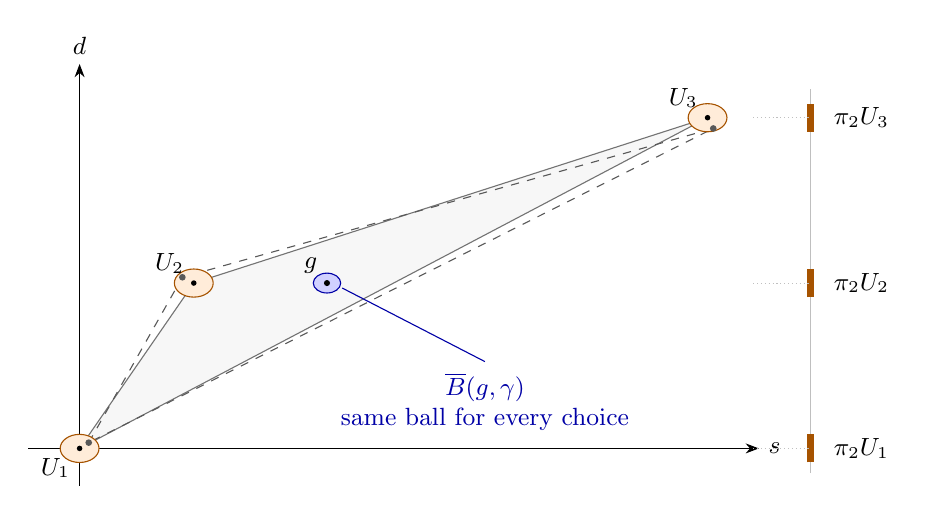
\begin{tikzpicture}[x=1.45cm,y=1.05cm,>=Stealth,
                    every node/.style={font=\small}]
 \coordinate (Vone) at (0,0);
 \coordinate (Vtwo) at (1,2);
 \coordinate (Vthree) at (5.5,4);
 \coordinate (G) at (2.166667,2);
 \coordinate (Aone) at (.08,.07);
 \coordinate (Atwo) at (.90,2.07);
 \coordinate (Athree) at (5.55,3.87);
 \draw[->] (-.45,0) -- (5.95,0) node[right] {$s$};
 \draw[->] (0,-.45) -- (0,4.65) node[above] {$d$};
 \fill[black!3] (Vone) -- (Vtwo) -- (Vthree) -- cycle;
 \draw[black!55] (Vone) -- (Vtwo) -- (Vthree) -- cycle;
 \draw[black!65,dashed] (Aone) -- (Atwo) -- (Athree) -- cycle;
 \foreach \point in {Vone,Vtwo,Vthree}{
  \filldraw[fill=orange!15,draw=orange!65!black] (\point) circle[radius=.17];
 }
 \foreach \point in {Vone,Vtwo,Vthree}{
  \fill (\point) circle[radius=1pt];
 }
 \foreach \point in {Aone,Atwo,Athree}{
  \fill[black!65] (\point) circle[radius=1.2pt];
 }
 \node[below left] at (Vone) {$U_1$};
 \node[above left] at (Vtwo) {$U_2$};
 \node[above left] at (Vthree) {$U_3$};
 \filldraw[fill=blue!18,draw=blue!65!black] (G) circle[radius=.12];
 \fill (G) circle[radius=1.1pt];
 \node[above left] at (G) {$g$};
 \draw[blue!65!black] (2.30,1.94) -- (3.55,1.05);
 \node[blue!65!black,anchor=north,align=center] at (3.55,1.03)
   {$\overline B(g,\gamma)$\\same ball for every choice};
 \draw[black!25] (6.4,-.30) -- (6.4,4.35);
 \foreach \height in {0,2,4}{
  \draw[orange!65!black,line width=2.4pt]
    (6.4,{\height-.17}) -- (6.4,{\height+.17});
  \draw[black!25,densely dotted] (5.9,\height) -- (6.4,\height);
 }
 \node[anchor=west] at (6.52,0) {$\pi_2U_1$};
 \node[anchor=west] at (6.52,2) {$\pi_2U_2$};
 \node[anchor=west] at (6.52,4) {$\pi_2U_3$};
\end{tikzpicture}
\caption{Schematic geometry of the three slope neighborhoods. The two
triangles illustrate different choices of one point from each $U_i$.
The choice of the neighborhoods guarantees
$\overline B(g,\gamma)\subset\conv\{u_1,u_2,u_3\}$ for every
$u_i\in U_i$, while $g$ belongs to the convex hull of no two neighborhoods.
Their density projections $\pi_2U_i$, where $\pi_2(s,d)=d$, are disjoint. The actual supporting
groups lie in $d\ge0$, although $U_1$ extends below that line.}
\label{fig:robust-triple}
\end{figure}


\begin{proposition}[Initial supporting triple]\label{prop:initial-triple}
For all sufficiently large \(t\), there are
\(\lambda_1\in B(\lambda_*,r_0/16)\) and nonempty compact convex sets
\(K_i^1\subset\overline B(v_i,\tau/2)\), \(i=1,2,3\), such that
\begin{equation}\label{eq:initial-triple}
 g\in\partial P_1^t(\lambda_1)
       =\conv\bigl(K_1^1\cup K_2^1\cup K_3^1\bigr).
\end{equation}
All vectors in the \(K_i^1\) have nonnegative density coordinate.
In particular \(\partial P_1^t(\lambda_1)\) contains
\(\overline B(g,\gamma)\).
\end{proposition}

\begin{proof}
The function \(P_*(y)-g\cdot y\) has its unique minimum at
\(\lambda_*\).  In fact
\[
 P_*(y)-P_*(\lambda_*)-g\cdot(y-\lambda_*)
 =\max_i(v_i-g)\cdot(y-\lambda_*)\ge\gamma_0|y-\lambda_*|
\]
for some \(\gamma_0>0\), because the triangle of the \(v_i\)
contains a ball about \(g\).
Minimize \(P_1^t(y)-g\cdot y\) over
\(\overline B(\lambda_*,r_0/16)\).
Lemma~\ref{lem:initial-transform} shows that all minimizers lie in
the interior for large \(t\) and converge to \(\lambda_*\) as
\(t\to\infty\).  Choose one and call it \(\lambda_1^t\).
Interior minimality gives \(g\in\partial P_1^t(\lambda_1^t)\).
It remains to locate the slopes generating this subdifferential.

We claim that any limit of gradients
\(\nabla P_1^{t_j}(\beta_j,h_j)\), at differentiability points with
\(t_j\to\infty\) and \((\beta_j,h_j)\to\lambda_*\), belongs to
\(\{v_1,v_2,v_3\}\).  Choose a maximizing density \(d_j\) at each
such point. Apply Lemma~\ref{lem:transform-support} with $Q=q_{t_j}$
and $a=A$, choosing
$e_j\in-\partial_\beta^+H_{t_j}(\beta_j,d_j)$.
With $z_j=h_j+\beta_jAd_j$, it gives
\begin{equation}\label{eq:initial-gradient}
 \nabla P_1^{t_j}(\beta_j,h_j)
            =\left(e_j+\frac{Ad_j^2}{2},d_j\right),
\end{equation}
and
\begin{equation}\label{eq:initial-joint-support}
 (e_j,d_j)\in\partial q_{t_j}(\beta_j,z_j).
\end{equation}
The shifted support controls the original first-coordinate slope $e_j$
before the explicit increment $Ad_j^2/2$ is added.
The maximizing densities are bounded by
Lemma~\ref{lem:initial-transform}; hence the \(z_j\) stay in a
compact interval.  The locally uniform limit \(q_*\) is independent
of \(\beta\), so every cluster of the subgradients in
\eqref{eq:initial-joint-support} has first coordinate zero.
Therefore \(e_j\to0\).  The same lemma puts every density cluster
in \(\{0,p,4p\}\), and \eqref{eq:initial-gradient} proves the claim.

Subgradients of \(P_1^t\) near \(\lambda_*\) are bounded uniformly
for large \(t\), by \eqref{eq:ideal-three-planes}.
If \(G_{P_1^t}(\lambda_1^t)\) were not contained in
\(\bigcup_i\overline B(v_i,\tau/2)\) for arbitrarily large \(t\),
choose such a sequence of reachable gradients.  Approximate each
by a gradient at a differentiability point within distance \(1/t\)
of \(\lambda_1^t\), with gradient error tending to zero.
A bounded subsequence then contradicts the preceding claim.
Thus, for all sufficiently large \(t\), the three intersections
\[
 G_{P_1^t}(\lambda_1^t)\cap\overline B(v_i,\tau/2)
\]
cover the reachable-gradient set.  Let \(K_i^1\) be their convex
hulls.  They are compact and remain inside their respective balls.
Formula~\eqref{eq:reachable-gradient-formula} gives the equality
in \eqref{eq:initial-triple}.  None of the three sets is empty:
otherwise \(g\) would lie in the convex hull of two of the larger
balls \(U_i\).  Their density coordinates are nonnegative because
\(P_1^t\) is nondecreasing in \(h\).

Finally, choose one point in each \(K_i^1\).  Their triangle contains
\(\overline B(g,\gamma)\) by the fixed geometry of the \(U_i\), and
is contained in \(\partial P_1^t(\lambda_1^t)\).
\end{proof}

Fix from now on one \(t\) satisfying \eqref{eq:t-choice} and
Proposition~\ref{prop:initial-triple}, and suppress its superscript
when writing \(P_1=\T_Aq_t\) and \(\lambda_1\).
We have obtained a corner for an ideal transform.  A physical
finite-range approximation can smooth that corner, so uniform
approximation alone will not finish the proof.  The next section
shows how a further small mean-field attraction restores the
three separated groups of supporting slopes while moving their
common supporting point only a controlled distance.

\section{Persistence under a small attractive perturbation}
\label{sec:convex}

The initial transform has three separated groups of supporting gradients.
We now show how to retain this structure when an ideal pressure is replaced
by a sufficiently accurate physical pressure and a smaller attractive
quadratic is added. The approximation error must be small compared with
the strength of that quadratic. The proof examines both operations at the
same scale; ordinary uniform convergence alone would not retain a corner.

Throughout this section, $t$ is fixed as in
Proposition~\ref{prop:initial-triple}. A physical pressure means a function
$Q=Q_\varphi$ with $\varphi$ in the class~\eqref{eq:physical-class}.
We use the following conclusions of
Propositions~\ref{prop:thermodynamics} and~\ref{prop:transform}:
$Q$ is finite, jointly convex, and
nondecreasing in $h$; its partial conjugate $H_Q(\beta,d)$ is finite and
concave in $\beta$ for every $d\geq0$; and the suprema defining
$\T_aQ$ are attained. On every compact subset of $\Omega$, their optimizing
densities are bounded uniformly over this physical class and over
$0\leq a\leq\min(1,A+1)$. These uniform bounds use the fixed value of $t$.
They are the only model-dependent bounds needed below.

For a nonempty compact convex set $K\subset\R^2$, define its support
function and its exposed faces by
\begin{equation}
 h_K(\xi)=\max_{v\in K}\xi\cdot v,
 \qquad
 F_\xi=\{v\in K:\xi\cdot v=h_K(\xi)\}.
 \label{eq:support-face}
\end{equation}
The face $F_0$ is the whole set $K$. Two facts about finite convex
functions will be used repeatedly. Locally uniform convergence bounds
subgradients on smaller compact subsets, and limits of subgradients at
converging points belong to the subdifferential of the limiting function.
Both statements follow directly from supporting inequalities and the
bound of a slope by the oscillation on a surrounding ball. In particular,
$\partial h_K(\xi)=F_\xi$. We also use the reachable-gradient identity
$\partial F(\lambda)=\conv G_F(\lambda)$ recalled in the preceding section.

\begin{lemma}[Persistence of three gradient groups]
\label{lem:persistence}
Let $W\subset\Omega$ be compact, let $P$ be finite and convex on $\Omega$,
and let $\lambda_0=(\beta_0,h_0)\in\operatorname{int}W$. Suppose that
\begin{equation}
 \partial P(\lambda_0)=K=\conv(K_1\cup K_2\cup K_3),
 \qquad B(g,\gamma)\subset K,
 \label{eq:persistence-input}
\end{equation}
where $g\in\R^2$, $\gamma>0$, and the $K_i$ are nonempty compact convex
sets whose projections onto the density coordinate are nonnegative and
strictly ordered. Let $\zeta>0$ be such that the sets
$K_i+\overline B(0,\zeta)$ still have disjoint density projections, and
$g$ lies outside the convex hull of any two of these enlarged sets.

There exist $S<\infty$ and $a_*>0$ with the following property. For every
$0<a<a_*$ and every physical pressure $Q$ satisfying
\begin{equation}
 \|Q-P\|_W\leq a^2,
 \label{eq:persistence-error}
\end{equation}
there is a point $\lambda'\in\operatorname{int}W$ with
$|\lambda'-\lambda_0|\leq Sa$ such that
\begin{equation}
 g\in\partial(\T_aQ)(\lambda')
   =\conv(J_1\cup J_2\cup J_3).
 \label{eq:persistence-output}
\end{equation}
Here each $J_i$ is nonempty, compact, and convex, has nonnegative density
projection, and satisfies $J_i\subset K_i+\overline B(0,\zeta)$.
The constants may depend on the displayed data and the fixed physical
class, but not on $Q$. We may require $a_*\leq\min(1,A+1)$.
\end{lemma}

\begin{proof}
We prove the conclusion along an arbitrary sequence $a_m\downarrow0$
and physical pressures $Q_m$ with
$\|Q_m-P\|_W\leq a_m^2$. The radius $S$ will be chosen from the fixed
limiting data. A contradiction argument will then supply one threshold
$a_*$ valid for all admissible $Q$.

\smallskip
\noindent\textit{The geometric effect of the quadratic.}
Write $\xi=(x,y)$ and $\pi_2(s,d)=d$. Define the finite convex function
\begin{equation}
 r(x,y)=\max_{(s,d)\in K}
       \left(xs+yd+\frac{\beta_0}{2}d^2\right)
 \label{eq:scaled-transform-limit-definition}
\end{equation}

This is the function that will arise when the attractive mass and the
distance to $\lambda_0$ tend to zero at the same scale. Before proving that
limit, we identify which points of $K$ can attain its maximum.
Every maximizer of
$\xi\cdot(s,d)+\beta_0d^2/2$ over $K$ belongs to one of the $K_i$.
Indeed, write such a maximizer as a finite convex combination
$v=\sum_j\theta_jv_j$, with $v_j=(s_j,d_j)\in\bigcup_iK_i$ and
positive weights. If two of the $d_j$ differ, strict convexity of the
quadratic gives
\[
 \xi\cdot v+\frac{\beta_0}{2}(\pi_2v)^2
   <\sum_j\theta_j\left(\xi\cdot v_j+
                                      \frac{\beta_0}{2}d_j^2\right)
   \leq r(\xi),
\]
contradicting maximality. All $d_j$ must therefore coincide. The disjoint
density projections put all $v_j$ in one $K_i$, and convexity of that
$K_i$ gives $v\in K_i$. 
Thus the positive quadratic rules out a maximizing mixture across the three
density groups. To use this observation for physical pressures, we must show
that limits of their transformed gradients are themselves maximizing points
of $K$; membership in the convex hull of such points would not suffice.

\smallskip
\noindent\textit{Step 1: the pressure at scale $a_m$.}
On the expanding open set
$\Omega_m=\{\xi\in\R^2:\lambda_0+a_m\xi\in\Omega\}$, put
\begin{equation}
 q_m(\xi)=
 \frac{Q_m(\lambda_0+a_m\xi)-P(\lambda_0)}{a_m}.
 \label{eq:scaled-pressure}
\end{equation}
Every fixed compact set of scaled coordinates is mapped into
$\operatorname{int}W$ for all sufficiently large $m$. On that compact
set, the difference between $q_m$ and the corresponding rescaling of $P$
is at most $a_m$. The rescaling of $P$ converges to its directional
derivative at $\lambda_0$, which is $h_K$. This convergence is uniform
on compact sets: the rescaled functions have a common local Lipschitz
bound, and their pointwise limits are the directional derivatives.
Consequently
\begin{equation}
 q_m\longrightarrow h_K
 \quad\text{locally uniformly on }\R^2.
 \label{eq:scaled-pressure-limit}
\end{equation}

The scaling preserves subgradient vectors:
\[
 \partial q_m(\xi)
   =\partial Q_m(\lambda_0+a_m\xi).
\]
It follows that, whenever $\xi_m\to\xi$ and
$v_m\in\partial Q_m(\lambda_0+a_m\xi_m)$, the vectors $v_m$ are bounded
and every limit belongs to $F_\xi$. To see the last assertion directly,
pass the supporting inequalities of $q_m$ to the limit. They give
$v\in\partial h_K(\xi)=F_\xi$. This observation applies to faces of any
dimension; no uniqueness of the supporting vector is assumed.

\smallskip
\noindent\textit{Step 2: the transform at the same scale.}
Put
\[
 B_m(\xi)=
 \frac{\T_{a_m}Q_m(\lambda_0+a_m\xi)-P(\lambda_0)}{a_m}.
\]
We will prove that
\begin{equation}
 B_m\longrightarrow r
 \quad\text{locally uniformly on }\R^2.
 \label{eq:scaled-transform-limit}
\end{equation}
To keep track of maximizing densities as well as function values, we use the slices of $K$.
For fixed $x\in\R$, define
\[
 k_x(d)=\max\{xs:(s,d)\in K\},
\]
with value $-\infty$ when $d$ is outside the density projection of $K$.
The function $k_x$ is upper semicontinuous and concave on its compact
interval of finite values. Partial conjugacy of the support function gives
\begin{equation}
 k_x(d)=\inf_{z\in\R}\bigl(h_K(x,z)-zd\bigr).
 \label{eq:slice-conjugacy}
\end{equation}
Indeed $h_K(x,z)=\sup_d(k_x(d)+zd)$; the reverse formula is concave
biconjugacy, or equivalently separation of the closed hypograph of $k_x$.

We will also retain the following information about optimizers: if
$\xi_m=(x_m,y_m)\to(x,y)$ and $d_m$ maximizes the transform at
$\lambda_0+a_m\xi_m$, then every limit $d$ of the $d_m$ satisfies
\begin{equation}
 d\in\pi_2K,
 \qquad
 r(x,y)=k_x(d)+yd+\frac{\beta_0}{2}d^2.
 \label{eq:scaled-optimizer}
\end{equation}

Write $\beta_m=\beta_0+a_mx_m$ and $h_m=h_0+a_my_m$.
The physical uniform bound on optimizing densities makes $(d_m)$
bounded. For every fixed $z\in\R$, Fenchel's inequality at
$(\beta_m,h_0+a_mz)$ gives
\begin{equation}
 B_m(\xi_m)\leq q_m(x_m,z)+(y_m-z)d_m
                     +\frac{\beta_m}{2}d_m^2.
 \label{eq:scaled-upper}
\end{equation}
This will yield the upper bound after taking a density limit and then
the infimum over $z$.

For the lower bound, choose $v_*=(s_*,d_*)\in K$ that attains the
maximum defining $r(x,y)$, and put $z=y+\beta_0d_*$. Comparing its value
with that at any $(s',d')\in K$ and completing the square gives
\begin{equation}
 x(s_*-s')+z(d_*-d')
       \geq\frac{\beta_0}{2}(d'-d_*)^2.
 \label{eq:strict-face-support}
\end{equation}
Thus $v_*\in F_{(x,z)}$, and every member of this face has density $d_*$.
Choose a full subgradient of $Q_m$ at $(\beta_m,h_0+a_mz)$, and denote
its density coordinate by $d'_m$. Step~1 shows that $d'_m\to d_*$;
nondecreasing dependence on $h$ gives $d'_m\geq0$. Fenchel equality at
$d'_m$ permits evaluation of the transformed objective and yields
\begin{align}
 B_m(\xi_m)
 &\geq q_m(x_m,z)+(y_m-z)d'_m
                       +\frac{\beta_m}{2}(d'_m)^2 \notag\\
 &\longrightarrow xs_*+yd_*+\frac{\beta_0}{2}d_*^2
   =r(x,y).
 \label{eq:scaled-lower}
\end{align}

Now pass to a subsequence in~\eqref{eq:scaled-upper} along which
$d_m\to d$. Taking the infimum over $z$ after the limit and using
\eqref{eq:slice-conjugacy} gives
\[
 \limsup_m B_m(\xi_m)
   \leq k_x(d)+yd+\frac{\beta_0}{2}d^2
   \leq r(x,y).
\]
The finite lower bound~\eqref{eq:scaled-lower} excludes
$d\notin\pi_2K$. Equality throughout proves
\eqref{eq:scaled-optimizer}. These arguments apply to every convergent
sequence $\xi_m$ in a fixed compact set. They therefore prove the uniform
convergence~\eqref{eq:scaled-transform-limit} as well.

We have identified the exact effect of an attraction of strength $a_m$
on the pressure at distance $O(a_m)$ from $\lambda_0$. The positive
quadratic in~\eqref{eq:scaled-transform-limit-definition} is now visible
at order one. We next use it to locate a nearby subdifferential containing
$g$ and to keep all of its reachable gradients within the three groups.

\smallskip
\noindent\textit{Step 3: a nearby point supporting $g$.}
By~\eqref{eq:persistence-input} and $\beta_0>0$,
\begin{equation}
 r(\xi)-g\cdot\xi
    \geq h_K(\xi)-g\cdot\xi
    \geq\gamma|\xi|.
 \label{eq:scaled-coercivity}
\end{equation}
Choose $S>0$ such that $\gamma S>r(0)+1$.
Let $\xi_m$ minimize $B_m(\xi)-g\cdot\xi$ on the closed ball
$\overline B(0,S)$. Uniform convergence on this ball and
\eqref{eq:scaled-coercivity} show that, for large $m$, all such minimizers
are interior: every boundary value exceeds the value at $0$. Every
limit of these minimizers is also interior. Hence, at
\[
 \lambda'_m=\lambda_0+a_m\xi_m,
\]
convex minimality gives
\begin{equation}
 g\in\partial(\T_{a_m}Q_m)(\lambda'_m),
 \qquad |\lambda'_m-\lambda_0|\leq Sa_m.
 \label{eq:nearby-support}
\end{equation}
For large $m$ these points lie in $\operatorname{int}W$.

\smallskip
\noindent\textit{Step 4: localization of every reachable gradient.}
Put $G_m=G_{\T_{a_m}Q_m}(\lambda'_m)$. We claim that, eventually,
\begin{equation}
 G_m\subset\bigcup_{i=1}^3
                  \left(K_i+\overline B(0,\zeta/2)\right).
 \label{eq:reachable-localization}
\end{equation}
Suppose otherwise, and choose $u_m\in G_m$ outside this union along a
subsequence. By the definition of a reachable gradient, there is a
differentiability point $\widehat\lambda_m$ of $\T_{a_m}Q_m$ such that
\[
 |\widehat\lambda_m-\lambda'_m|<a_m^2,
 \qquad
 |\nabla(\T_{a_m}Q_m)(\widehat\lambda_m)-u_m|<1/m.
\]
Write $\widehat\lambda_m=\lambda_0+a_m\widehat\xi_m$, with
$\widehat\xi_m=(\widehat x_m,\widehat y_m)$.
The scaled points remain in a fixed compact set. Moreover, scaling
preserves the gradients of the transforms:
\[
 \nabla B_m(\widehat\xi_m)
       =\nabla(\T_{a_m}Q_m)(\widehat\lambda_m).
\]
Their boundedness thus follows from the local uniform convex convergence
in~\eqref{eq:scaled-transform-limit}. After passing to a subsequence,
assume
\[
 \xi_m\to\xi=(x,y),\qquad
 \widehat\xi_m\to\xi,\qquad u_m\to u=(s,d).
\]

Let $d_m$ be any maximizing density at
$\widehat\lambda_m=(\widehat\beta_m,\widehat h_m)$. Apply
Lemma~\ref{lem:transform-support} with $Q=Q_m$ and $a=a_m$.
Because $H_{Q_m}(\,\cdot\,,d_m)$ is finite and concave, we can choose
$e_m\in-\partial_\beta^+H_{Q_m}(\widehat\beta_m,d_m)$; the lemma gives
\begin{equation}
 \nabla(\T_{a_m}Q_m)(\widehat\lambda_m)
       =\left(e_m+\frac{a_m}{2}d_m^2,d_m\right),
 \label{eq:transformed-gradient}
\end{equation}
and
\begin{equation}
 (e_m,d_m)\in
 \partial Q_m\bigl(\widehat\beta_m,
                   \widehat h_m+\widehat\beta_m a_md_m\bigr).
 \label{eq:full-gradient-support}
\end{equation}
In particular $d_m\to d$, and the first-coordinate increment tends to zero.
The argument on the right has scaled coordinates
\[
 \left(\widehat x_m,
       \widehat y_m+\widehat\beta_m d_m\right)
   \longrightarrow\eta=(x,y+\beta_0d).
\]
Equations~\eqref{eq:transformed-gradient} and
\eqref{eq:full-gradient-support}, together with Step~1, show that
$u\in F_\eta$.

By~\eqref{eq:scaled-optimizer}, there is a point
$v_*=(s_*,d)\in K$ that maximizes the expression defining $r(x,y)$.
Equation~\eqref{eq:strict-face-support} shows that $v_*\in F_\eta$ as
well. The vectors $u$ and $v_*$ have the same density and the same value
against $\eta$, so $xs=xs_*$. Consequently $u$ itself maximizes that
expression. This conclusion also holds when $x=0$; an exposed face need
not be a singleton.

Since $u$ is a maximizer, the geometric observation at the start of the proof
puts $u$ in one of the $K_i$. This contradicts the choice of $u_m$ outside
the fixed $\zeta/2$ neighborhoods. This proves
\eqref{eq:reachable-localization}.

\smallskip
\noindent\textit{Step 5: the three groups and a uniform threshold.}
Define
\[
 J_{i,m}=\conv\left(G_m\cap
                 \left(K_i+\overline B(0,\zeta/2)\right)\right).
\]
Reachable-gradient sets are compact. Hence every nonempty $J_{i,m}$ is
compact and convex, and lies in $K_i+\overline B(0,\zeta/2)$.
The reachable-gradient identity and
\eqref{eq:reachable-localization} give
\[
 \partial(\T_{a_m}Q_m)(\lambda'_m)
       =\conv(J_{1,m}\cup J_{2,m}\cup J_{3,m}).
\]
None of the three sets is empty: otherwise
\eqref{eq:nearby-support} would put $g$ in the convex hull of two of the
allowed enlarged groups. The density coordinate of every reachable
gradient is nonnegative because $\T_{a_m}Q_m$ is nondecreasing in $h$.
Thus the $J_{i,m}$ have all the asserted properties.

We have proved the conclusion for all sufficiently large indices along
every sequence $a_m\downarrow0$, with the same radius $S$. If no uniform
threshold $a_*$ existed, one could choose a sequence of counterexamples
with $a_m\downarrow0$, contradicting what was just proved. Decrease
$a_*$ if necessary so that $a_*\leq\min(1,A+1)$ and
$\lambda_0+\overline B(0,Sa_*)\subset\operatorname{int}W$.
This completes the proof.
\end{proof}

The lemma preserves the three groups even when they contain curved
families of supporting vectors. Its use in the construction is now
precise: an approximation with error at most $a^2$ can be followed by an
attraction of mass $a$, while moving the supporting point by at most
$Sa$ and enlarging each group by an arbitrarily prescribed amount.

\section{One potential and a common temperature singularity}\label{sec:construction}
We now replace each ideal quadratic attraction by an actual radial kernel and
retain a common ball of supporting slopes. Throughout this section, $t$ is
fixed at a value supplied by Proposition~\ref{prop:initial-triple}; it will
never tend to infinity again. All pressure estimates therefore use the
fixed-$t$ constants proved above. The ideal pressures carry the ball of
supporting slopes, while their physical approximations become the references
for the next step.

\subsection{Choose the next mass before the current range}
Recall the objects supplied by Proposition~\ref{prop:initial-triple}:
$A=3/(2p)$, $q_0=Q_{\psi_t}$, $P_1=T_Aq_0$, the point
$\lambda_*=(1,-3/4)$, a closed ball $W$ of radius $r_0=1/4$ about
$\lambda_*$, three small neighborhoods $U_i$ of the slope vectors $v_i$, and
$g=(v_1+v_2+v_3)/3$. Every triangle with one vertex in each $U_i$ contains
the same ball $\overline B(g,\gamma)$, for some $\gamma>0$.
The initial groups satisfy
$K_i^1\subset\overline B(v_i,\tau/2)$, whereas
$U_i=\overline B(v_i,4\tau)$.
Put $\sigma_1=A$. Choose positive sequences $\zeta_n$ and $\ell_n$ such that
\begin{equation}\label{eq:budgets}
 \sum_{n\ge1}\zeta_n<\tau,
 \qquad \sum_{n\ge1}\ell_n<r_0/16.
\end{equation}
The quantities $\ell_n$ bound displacements in the $(\beta,h)$ plane; they are
unrelated to the side lengths of particle boxes.

Suppose that the finite-range potential and the next ideal pressure have
already been defined by
\begin{align*}
 \varphi_{n-1}&=\psi_t-t\sum_{k<n}\sigma_k w_{R_k},
 &q_{n-1}&=Q_{\varphi_{n-1}},
 &P_n&=T_{\sigma_n}q_{n-1}.
\end{align*}
The induction maintains a point $\lambda_n\in\operatorname{int}W$ and
nonempty compact convex sets $K_i^n$ such that
\begin{equation}\label{eq:inductive-slopes}
 g\in\partial P_n(\lambda_n)
   =\conv\bigcup_{i=1}^3K_i^n,
 \qquad
 K_i^n\subset\overline B\left(v_i,\frac\tau2+
                          \sum_{k<n}\zeta_k\right),
\end{equation}
and every point in $K_i^n$ has nonnegative second coordinate. The geometric
choice of the $U_i$ gives
\begin{equation}\label{eq:common-ball}
 \overline B(g,\gamma)\subset\partial P_n(\lambda_n).
\end{equation}
The enlarged groups $K_i^n+\overline B(0,\zeta_n)$ lie in $U_i$;
their density projections are disjoint, and the convex hull of any two of
them does not contain $g$.

Apply Lemma~\ref{lem:persistence} to $P_n$, $\lambda_n$, and tolerance
$\zeta_n$. Denote its constants by $S_n$ and $a_n^*>0$. First choose
\begin{equation}\label{eq:choose-mass}
 0<\sigma_{n+1}<
 \min\left\{a_n^*,\frac{\ell_n}{\max\{1,S_n\}},2^{-n-1}\right\}.
\end{equation}
Only after this choice, select $R_n>4$, with $R_n>R_{n-1}+1$ for $n>1$,
so large that Proposition~\ref{prop:kac}, applied to the fixed finite-range
reference $\varphi_{n-1}$, gives
\begin{align}
 \varphi_n&=\varphi_{n-1}-t\sigma_nw_{R_n},
 &q_n&=Q_{\varphi_n},\notag\\
 \|q_n-P_n\|_W&\le\min\{\sigma_{n+1}^2,2^{-n}\}.
 \label{eq:choose-range}
\end{align}
The physical class is respected because
$\sum_{k\ge2}\sigma_k<1$, so every partial sum of the masses is at most
$A+1$. Lemma~\ref{lem:persistence} now applies to the physical pressure
$q_n$ with perturbation size $a=\sigma_{n+1}$. It produces
$P_{n+1}=T_{\sigma_{n+1}}q_n$, a point $\lambda_{n+1}$, and groups
$K_i^{n+1}$ satisfying
\[
 |\lambda_{n+1}-\lambda_n|\le\ell_n,
 \qquad K_i^{n+1}\subset K_i^n+\overline B(0,\zeta_n).
\]
This verifies \eqref{eq:inductive-slopes} at the next stage.
The initial location and \eqref{eq:budgets} keep every $\lambda_n$ in
$B(\lambda_*,r_0/8)$. Thus the construction continues indefinitely.

The order in \eqref{eq:choose-mass}--\eqref{eq:choose-range} is essential.
The next attractive mass sets the required precision for approximating the
current ideal pressure. No uniform convergence rate for the Kac limit as the
reference range changes is needed: that reference is fixed before each new
range is chosen.

\subsection{The final radial interaction}
Define
\begin{equation}\label{eq:final-potential}
 \Phi(x)=\psi_t(x)-t\sum_{j=1}^{\infty}\sigma_jw_{R_j}(x).
\end{equation}
Since $R_j\ge1$ and $\sum_j\sigma_j<\infty$, the attractive series
converges uniformly and in $L^1(\R^3)$. It is radial and nonnegative before
subtraction. Consequently $\Phi$ is Borel measurable, finite and locally
bounded away from the origin, and has the same divergence at the origin as
$\psi_t$. The core vanishes for $|x|\ge1$, so the $L^1$ convergence gives
\[
 4\pi\int_1^\infty r^2|\phi(r)|\dd r
 =\int_{|x|\ge1}|\Phi(x)|\dd x<\infty.
\]
The compact support of $w$ also gives, for $r\ge1$,
\[
 r^3|\phi(r)|\le t\|w\|_\infty\sum_{R_j\ge r}\sigma_j
 \longrightarrow0.
\]
This estimates the tail without imposing any power-law relation between
$\sigma_j$ and $R_j$. No bound of order $r^{-3-\varepsilon}$ for a fixed
$\varepsilon>0$ is established by these choices.
Because $R_1>4$ and $w$ is continuous and strictly positive on the ball of
radius $1/2$, its first attraction alone has a positive lower bound on
$1\le|x|\le2$. As $\sigma_1=A>0$,
\[
 \Phi(x)\le -tA R_1^{-3}
            \min_{|y|\le 2/R_1}w(y)<0
 \qquad(1\le|x|\le2).
\]
Finally, Proposition~\ref{prop:stability} applies to the infinite sum and
gives $U_N^\Phi\ge-B_0N$. Thus \eqref{eq:final-potential} satisfies every
admissibility condition in Section~\ref{sec:introduction}.

Write $Q_\infty=Q_\Phi$ and $H_\infty=H_\Phi$ for the actual pressure and
canonical limit of this potential. Their existence, finiteness, and duality
follow from Proposition~\ref{prop:thermodynamics}. The range-uniform tail
estimate, Proposition~\ref{prop:tail}, and \eqref{eq:choose-range} imply
\begin{equation}\label{eq:physical-pressure-limit}
 \|Q_\infty-P_n\|_W
 \le C_W\sum_{k>n}\sigma_k+\min\{\sigma_{n+1}^2,2^{-n}\}
 \longrightarrow0.
\end{equation}
This estimate identifies the limiting function with the pressure of the
single potential \eqref{eq:final-potential}.

\subsection{Pass the ball of slopes to the physical pressure}
The summable displacement bounds imply
$\lambda_n\to\lambda_c=(\beta_c,h_c)$, with
$\lambda_c\in B(\lambda_*,r_0/8)$.
Fix any $v\in\overline B(g,\gamma)$.
By \eqref{eq:common-ball}, for every $\lambda\in\operatorname{int}W$,
\[
 P_n(\lambda)\ge P_n(\lambda_n)+v\cdot(\lambda-\lambda_n).
\]
Letting $n\to\infty$ in this inequality using
\eqref{eq:physical-pressure-limit} gives a supporting inequality for
$Q_\infty$ at $\lambda_c$ on $\operatorname{int}W$.
Such a local support is global on the convex domain
$\Omega=(0,\infty)\times\R$. Indeed, for any $\lambda\in\Omega$, a short
initial portion of the segment from $\lambda_c$ to $\lambda$ lies in
$\operatorname{int}W$; combining its supporting inequality with convexity
of $Q_\infty$ gives the inequality at $\lambda$. Hence
\begin{equation}\label{eq:limit-ball}
 \overline B(g,\gamma)\subset\partial Q_\infty(\lambda_c).
\end{equation}
The same ball, rather than singularity alone, is the information that survives
all finite-range approximations.

\subsection{A common critical point for an open interval of densities}
The center density is determined by the original triangle:
\begin{equation}\label{eq:fixed-density}
 \rho_*=g_2=\frac{0+p+4p}{3}=\frac{5p}{3}>0.
\end{equation}
Set
\[
 \delta_\rho=\min\{\gamma/2,\rho_*/2\},\qquad
 I=(\rho_*-\delta_\rho,\rho_*+\delta_\rho).
\]
This nonempty interval lies in $(0,\infty)$ and is independent of inverse
temperature. Fix any $\rho\in I$. The vectors
\[
 w_-=(g_1-\gamma/2,\rho),\qquad
 w_+=(g_1+\gamma/2,\rho)
\]
have distance less than $\gamma$ from $g$, so both belong to
$\partial Q_\infty(\beta_c,h_c)$ by \eqref{eq:limit-ball}.
Figure~\ref{fig:fixed-density} shows the central slice; the same argument
applies to every slice at a density in $I$.

\begin{figure}[hbp]
\centering
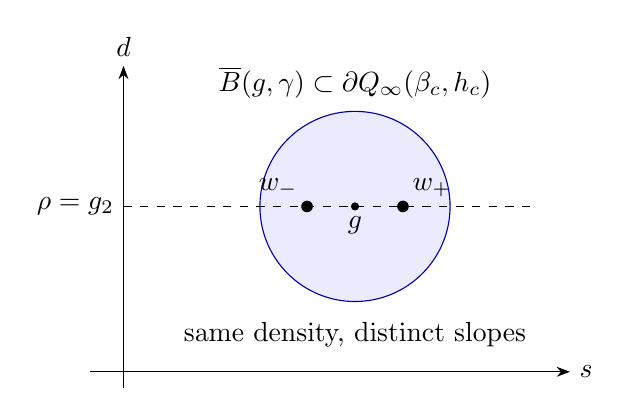
\begin{tikzpicture}[scale=1.05,>=Stealth]
 \draw[->] (-0.4,0) -- (5.4,0) node[right] {$s$};
 \draw[->] (0,-0.2) -- (0,3.7) node[above] {$d$};
 \fill[blue!8] (2.8,2) circle (1.15);
 \draw[blue!65!black] (2.8,2) circle (1.15);
 \draw[dashed] (0,2) node[left] {$\rho=g_2$} -- (5.0,2);
 \fill (2.8,2) circle (1.4pt) node[below] {$g$};
 \fill (2.22,2) circle (2pt) node[above left] {$w_-$};
 \fill (3.38,2) circle (2pt) node[above right] {$w_+$};
 \node[align=center] at (2.8,0.45) {same density, distinct slopes};
 \node at (2.8,3.5) {$\overline B(g,\gamma)\subset\partial Q_\infty(\beta_c,h_c)$};
\end{tikzpicture}
\caption{The horizontal slice of the preserved subgradient ball gives two
supporting vectors with the same density coordinate. Partial conjugacy turns
their distinct first coordinates into distinct canonical supergradients in
inverse temperature.}\label{fig:fixed-density}
\end{figure}

To obtain the temperature jump, take any $(s,\rho)$ in that subdifferential.
Restricting the
supporting inequality to $\beta=\beta_c$ gives Fenchel equality
\[
 H_\infty(\beta_c,\rho)=h_c\rho-Q_\infty(\beta_c,h_c).
\]
The full inequality, at an arbitrary $(\beta,h)\in\Omega$, rearranges to
\[
 h\rho-Q_\infty(\beta,h)
 \le H_\infty(\beta_c,\rho)-s(\beta-\beta_c).
\]
Taking the supremum over $h$ yields
\begin{equation}\label{eq:canonical-support}
 H_\infty(\beta,\rho)
 \le H_\infty(\beta_c,\rho)-s(\beta-\beta_c),\qquad \beta>0.
\end{equation}
Thus $-s$ is a supergradient of the finite concave function
$H_\infty(\cdot,\rho)$. For a finite concave function at an interior point,
every supergradient lies between the right and left derivatives. Applying
this to $w_-$ and $w_+$ gives
\begin{equation}\label{eq:derivative-jump}
 D_\beta^-H_\infty(\beta_c,\rho)
 -D_\beta^+H_\infty(\beta_c,\rho)\ge\gamma>0.
\end{equation}
Both derivatives are finite because $\beta_c$ is interior to the interval
of finiteness of this concave function.

The normalization \eqref{eq:free-energy-normalization} gives
$f_\Phi(\beta,\rho)=tH_\infty(\beta,\rho)/\beta$. Continuity and the
one-sided product rule therefore give the explicit uniform bound
\[
 D_\beta^- f_\Phi(\beta_c,\rho)
 -D_\beta^+ f_\Phi(\beta_c,\rho)
 =\frac{t}{\beta_c}\left(
 D_\beta^-H_\infty(\beta_c,\rho)
 -D_\beta^+H_\infty(\beta_c,\rho)\right)
 \ge\frac{t\gamma}{\beta_c}>0.
\]
The all-sequence canonical limit supplies
\eqref{eq:free-energy-definition} with $N_L=\lfloor\rho L^3\rfloor$
for every $\beta>0$ and every $\rho>0$. The location of $\lambda_c$
gives $\beta_c\in(1/2,3/2)$. Since the choice of $\rho\in I$ was arbitrary,
this proves Theorem~\ref{thm:main} with one potential and one critical point.

\appendix
\section{Elementary convex facts used in the proof}\label{app:convex-facts}
This appendix proves the finite-dimensional convex facts needed for the
pressure limits and the persistence argument. These are special cases of the
convex convergence, conjugacy, and reachable-gradient results in
\cite[Corollary~7.18 and Theorems~11.1 and 9.61]{RockafellarWets1998}. The proofs below
make their exact hypotheses explicit. Lebesgue measure and its Fubini theorem
are used only to locate ordinary differentiability points of a planar convex
function.

\begin{lemma}[Local convex convergence]\label{lem:elementary-convex-convergence}
Let $O\subset\R^m$ be open and convex. A finite convex function $F$ on $O$
is locally Lipschitz and has a nonempty compact subdifferential at every
point of $O$. Its subgradients are bounded on compact subsets. If finite
convex functions $F_n$ converge pointwise on $O$ to a finite function $F$,
then $F$ is convex and the convergence is locally uniform. Moreover, if
$x_n\to x\in O$, $F_n\to F$ locally uniformly, and
$v_n\in\partial F_n(x_n)$, then $(v_n)$ is bounded and every limit belongs
to $\partial F(x)$.
\end{lemma}

\begin{proof}
Choose a cube with center $c$ whose concentric enlargement lies in $O$.
Convexity bounds a function above on the larger cube by its values at the
vertices. The inequality
$F(y)\ge 2F(c)-F(2c-y)$ then bounds it below on a smaller concentric cube.
On a still smaller cube, extend any chord by a fixed positive distance in
both directions while remaining in the bounded region. Monotonicity of
one-dimensional convex secant slopes bounds the difference quotient on the
original chord by its surrounding oscillation divided by that distance.
This proves local Lipschitz continuity. In the sequence assertion, the
finitely many vertex values and the center value are uniformly bounded by
pointwise convergence, so the same argument gives a common local Lipschitz
constant. A finite net of points on each compact set upgrades pointwise to
uniform convergence. Passing convexity inequalities to limits proves
convexity of $F$.

Here is also a direct supporting-plane construction. Separate a point
strictly below the epigraph from that convex epigraph, let the point tend to
$(x,F(x))$, and normalize the separating normals. Separation in finite
dimensions follows by projecting an exterior point onto a closed convex set:
if $z$ is its nearest point, expansion of the squared distance along
$z+\theta(y-z)$ gives the separating inequality. One can restrict the
epigraph to a closed neighborhood of $x$ before applying this construction.
A limiting normal has a nonzero vertical component: a horizontal supporting
normal would separate $x$ from an open neighborhood of $x$, which is
impossible. Division by that component produces a local affine minorant
through $(x,F(x))$. Convexity extends it to all of $O$ by considering the
initial portion of the segment from $x$ to any other point. Thus
$\partial F(x)$ is nonempty.

If $v\in\partial F(x)$ and $x\pm re_j\in O$, the supporting inequalities
bound $|v\cdot e_j|$ by the oscillation of $F$ divided by $r$.
Uniform oscillation on a surrounding compact set bounds all subgradients
at points in a smaller compact set. Subdifferentials are closed by their
defining inequalities, hence compact. The same bounds apply to $F_n$ under
local uniform convergence. Passing
$F_n(y)\ge F_n(x_n)+v_n\cdot(y-x_n)$ to a convergent subsequence proves the
last assertion.
\end{proof}

\begin{lemma}[One-dimensional conjugacy]\label{lem:elementary-conjugacy}
Let $u:\R\to\R\cup\{+\infty\}$ be proper, lower semicontinuous, and convex,
with a domain having nonempty interior. Then
\[
 u(d)=\sup_{h\in\R}\{hd-u^*(h)\},\qquad
 u^*(h)=\sup_{d\in\R}\{hd-u(d)\}.
\]
At a finite point $d$, equality $u(d)+u^*(h)=hd$ holds precisely when
$u(d')\ge u(d)+h(d'-d)$ for every $d'$. In particular, if $K\subset\R^2$
is nonempty compact convex with a density projection of positive length,
then for every $x\in\R$,
\[
 \max\{xs:(s,d)\in K\}
 =\inf_{z\in\R}\{h_K(x,z)-zd\},
\]
where the maximum is $-\infty$ outside that projection.
\end{lemma}

\begin{proof}
At every interior point of the domain, a slope between the left and right
convex derivatives gives an affine minorant. Hence $u$ has at least one
affine minorant $\ell_0$. To obtain enough such minorants, fix a point
$(d,a)$ strictly below the closed epigraph of $u$. Strict separation, by
the projection argument in the preceding proof, yields an affine inequality
\[
 A d'+B y\ge c>A d+B a\qquad(y\ge u(d')).
\]
Necessarily $B\ge0$. If $B>0$, division gives an affine minorant of $u$
whose value at $d$ exceeds $a$. If $B=0$, add a sufficiently small positive
multiple of the valid inequality $y\ge\ell_0(d')$; the resulting
inequality has positive vertical coefficient and still strictly separates
$(d,a)$. This also gives an affine minorant exceeding $a$ at $d$.
Since every point below the epigraph is so separated, $u$ is the supremum
of its affine minorants, including at boundary and exterior points of its
domain. Among affine minorants of slope $h$, the largest is
$d\mapsto hd-u^*(h)$, which proves biconjugacy. Rearranging the definition
of $u^*$ proves the equality criterion.

For the last assertion, put
$k_x(d)=\max\{xs:(s,d)\in K\}$. Compactness and convexity of $K$ make
$k_x$ upper semicontinuous and concave on its compact projection interval.
Thus $-k_x$, extended by $+\infty$, satisfies the preceding hypotheses.
The identity $h_K(x,z)=\sup_d(k_x(d)+zd)$ and biconjugacy give the formula.
\end{proof}

\begin{lemma}[Directional and reachable gradients]\label{lem:reachable-local}
Let $F$ be finite and convex on an open convex subset $O\subset\R^2$.
For $x\in O$, let $G_F(x)$ be the limits of gradients at differentiability
points tending to $x$. Then $G_F(x)$ is nonempty compact and
\[
 \partial F(x)=\conv G_F(x).
\]
For every $e\in\R^2$,
\[
 \lim_{a\downarrow0}\frac{F(x+ae)-F(x)}a
 =\max_{v\in\partial F(x)}v\cdot e.
\]
The rescaled functions in this last display converge uniformly for $e$ in
compact subsets of $\R^2$.
\end{lemma}

\begin{proof}
On every coordinate line, a one-dimensional convex function has equal left
and right derivatives except at countably many points: both derivatives
are monotone, and each strict gap contains a distinct rational number.
Fubini's theorem therefore implies that both coordinate partial derivatives
of $F$ exist almost everywhere. At such a point, every subgradient has these
two coordinates, so the subdifferential is a singleton, say $\{v\}$.
This implies differentiability. Indeed, for small $u$ choose
$v_u\in\partial F(x+u)$. Local boundedness and closedness of subgradients
show $v_u\to v$, and the two supporting inequalities give
\[
 v\cdot u\le F(x+u)-F(x)\le v_u\cdot u.
\]
Their difference is $o(|u|)$. Thus differentiability points have full
measure, in particular they are dense.

Local boundedness and diagonal subsequences show that $G_F(x)$ is nonempty
and compact. Each of its elements is in $\partial F(x)$ by the limiting
support inequality. Conversely, take $p\in\partial F(x)$ and a direction
$e$. Choose differentiability points
$y_j=x+a_je+o(a_j)$, with $a_j\downarrow0$. This is possible by density,
for example with error less than $a_j^2$. Adding the supporting
inequalities at $x$ and $y_j$ gives
\[
 (\nabla F(y_j)-p)\cdot(y_j-x)\ge0.
\]
After passing to a bounded-gradient subsequence and dividing by $a_j$,
one obtains $v\in G_F(x)$ with $v\cdot e\ge p\cdot e$.
Thus $G_F(x)$ and $\partial F(x)$ have the same support function.
In the plane the convex hull of a compact set is compact: any convex
combination can be reduced to three terms by eliminating an affine
dependence among four or more points. Separation therefore proves
$\partial F(x)=\conv G_F(x)$.

Finally, the convex secant slope in the last assertion has a limit as
$a\downarrow0$. Supporting inequalities at $x$ give the lower bound
$v\cdot e$ for every $v\in\partial F(x)$. Choose instead
$v_a\in\partial F(x+ae)$; the reverse supporting inequality bounds the
same secant slope above by $v_a\cdot e$. A bounded subsequence of $v_a$
converges to an element of $\partial F(x)$, proving the claimed equality.
The local Lipschitz constant for $F$ gives a common Lipschitz constant
in $e$ for all sufficiently small rescalings on any fixed compact set.
A finite-net argument then proves uniform convergence there.
\end{proof}

\bibliographystyle{plain}
\bibliography{refs}
\end{document}
